\documentclass[
  man,
  floatsintext,
  longtable,
  nolmodern,
  notxfonts,
  notimes,
  colorlinks=true,linkcolor=blue,citecolor=blue,urlcolor=blue]{apa7}

\usepackage{amsmath}
\usepackage{amssymb}



\usepackage[bidi=default]{babel}
\babelprovide[main,import]{english}


% get rid of language-specific shorthands (see #6817):
\let\LanguageShortHands\languageshorthands
\def\languageshorthands#1{}

\RequirePackage{longtable}
\RequirePackage{threeparttablex}

\makeatletter
\renewcommand{\paragraph}{\@startsection{paragraph}{4}{\parindent}%
	{0\baselineskip \@plus 0.2ex \@minus 0.2ex}%
	{-.5em}%
	{\normalfont\normalsize\bfseries\typesectitle}}

\renewcommand{\subparagraph}[1]{\@startsection{subparagraph}{5}{0.5em}%
	{0\baselineskip \@plus 0.2ex \@minus 0.2ex}%
	{-\z@\relax}%
	{\normalfont\normalsize\bfseries\itshape\hspace{\parindent}{#1}\textit{\addperi}}{\relax}}
\makeatother




\usepackage{longtable, booktabs, multirow, multicol, colortbl, hhline, caption, array, float, xpatch}
\setcounter{topnumber}{2}
\setcounter{bottomnumber}{2}
\setcounter{totalnumber}{4}
\renewcommand{\topfraction}{0.85}
\renewcommand{\bottomfraction}{0.85}
\renewcommand{\textfraction}{0.15}
\renewcommand{\floatpagefraction}{0.7}

\usepackage{tcolorbox}
\tcbuselibrary{listings,theorems, breakable, skins}
\usepackage{fontawesome5}

\definecolor{quarto-callout-color}{HTML}{909090}
\definecolor{quarto-callout-note-color}{HTML}{0758E5}
\definecolor{quarto-callout-important-color}{HTML}{CC1914}
\definecolor{quarto-callout-warning-color}{HTML}{EB9113}
\definecolor{quarto-callout-tip-color}{HTML}{00A047}
\definecolor{quarto-callout-caution-color}{HTML}{FC5300}
\definecolor{quarto-callout-color-frame}{HTML}{ACACAC}
\definecolor{quarto-callout-note-color-frame}{HTML}{4582EC}
\definecolor{quarto-callout-important-color-frame}{HTML}{D9534F}
\definecolor{quarto-callout-warning-color-frame}{HTML}{F0AD4E}
\definecolor{quarto-callout-tip-color-frame}{HTML}{02B875}
\definecolor{quarto-callout-caution-color-frame}{HTML}{FD7E14}

%\newlength\Oldarrayrulewidth
%\newlength\Oldtabcolsep


\usepackage{hyperref}




\providecommand{\tightlist}{%
  \setlength{\itemsep}{0pt}\setlength{\parskip}{0pt}}
\usepackage{longtable,booktabs,array}
\usepackage{calc} % for calculating minipage widths
% Correct order of tables after \paragraph or \subparagraph
\usepackage{etoolbox}
\makeatletter
\patchcmd\longtable{\par}{\if@noskipsec\mbox{}\fi\par}{}{}
\makeatother
% Allow footnotes in longtable head/foot
\IfFileExists{footnotehyper.sty}{\usepackage{footnotehyper}}{\usepackage{footnote}}
\makesavenoteenv{longtable}

\usepackage{graphicx}
\makeatletter
\newsavebox\pandoc@box
\newcommand*\pandocbounded[1]{% scales image to fit in text height/width
  \sbox\pandoc@box{#1}%
  \Gscale@div\@tempa{\textheight}{\dimexpr\ht\pandoc@box+\dp\pandoc@box\relax}%
  \Gscale@div\@tempb{\linewidth}{\wd\pandoc@box}%
  \ifdim\@tempb\p@<\@tempa\p@\let\@tempa\@tempb\fi% select the smaller of both
  \ifdim\@tempa\p@<\p@\scalebox{\@tempa}{\usebox\pandoc@box}%
  \else\usebox{\pandoc@box}%
  \fi%
}
% Set default figure placement to htbp
\def\fps@figure{htbp}
\makeatother


% definitions for citeproc citations
\NewDocumentCommand\citeproctext{}{}
\NewDocumentCommand\citeproc{mm}{%
  \begingroup\def\citeproctext{#2}\cite{#1}\endgroup}
\makeatletter
 % allow citations to break across lines
 \let\@cite@ofmt\@firstofone
 % avoid brackets around text for \cite:
 \def\@biblabel#1{}
 \def\@cite#1#2{{#1\if@tempswa , #2\fi}}
\makeatother
\newlength{\cslhangindent}
\setlength{\cslhangindent}{1.5em}
\newlength{\csllabelwidth}
\setlength{\csllabelwidth}{3em}
\newenvironment{CSLReferences}[2] % #1 hanging-indent, #2 entry-spacing
 {\begin{list}{}{%
  \setlength{\itemindent}{0pt}
  \setlength{\leftmargin}{0pt}
  \setlength{\parsep}{0pt}
  % turn on hanging indent if param 1 is 1
  \ifodd #1
   \setlength{\leftmargin}{\cslhangindent}
   \setlength{\itemindent}{-1\cslhangindent}
  \fi
  % set entry spacing
  \setlength{\itemsep}{#2\baselineskip}}}
 {\end{list}}
\usepackage{calc}
\newcommand{\CSLBlock}[1]{\hfill\break\parbox[t]{\linewidth}{\strut\ignorespaces#1\strut}}
\newcommand{\CSLLeftMargin}[1]{\parbox[t]{\csllabelwidth}{\strut#1\strut}}
\newcommand{\CSLRightInline}[1]{\parbox[t]{\linewidth - \csllabelwidth}{\strut#1\strut}}
\newcommand{\CSLIndent}[1]{\hspace{\cslhangindent}#1}


\usepackage[nolongtablepatch]{lineno}
\linenumbers



\usepackage{newtx}

\defaultfontfeatures{Scale=MatchLowercase}
\defaultfontfeatures[\rmfamily]{Ligatures=TeX,Scale=1}





\title{Meta-analysis of the Interoceptive Accuracy Scale (IAS) Structure
and its Subjective Correlates}


\shorttitle{IAS Meta-analysis}


\usepackage{etoolbox}






\author{Ana Neves}



\affiliation{
{School of Psychology, University of Sussex}}




\leftheader{Neves}



\abstract{Blabla the abstract blabla.}

\keywords{keyword1, keyword2, keyword3}

\authornote{\par{\addORCIDlink{Ana Neves}{0009-0006-0020-7599}} 

\par{     \begin{tcolorbox}[enhanced jigsaw, colback=white, colframe=quarto-callout-note-color-frame, leftrule=.75mm, opacityback=0, arc=.35mm, toprule=.15mm, breakable, rightrule=.15mm, left=2mm, bottomrule=.15mm]

\end{tcolorbox}

This preprint is a non-peer-reviewed work from the
\href{https://realitybending.github.io/}{\textbf{Reality Bending Lab}}.
\begin{center}

\includegraphics[width=0.2\linewidth,height=\textheight,keepaspectratio]{manuscript_files/mediabag/ReBeL_LogoOnly_hu114.png}
\end{center}  Author roles were classified using the Contributor Role Taxonomy (CRediT; https://credit.niso.org/) as follows: Ana
Neves:   Project administration, Data curation, Formal
Analysis, Investigation, Visualization, Writing -- original
draft, Writing -- review \& editing}
\par{Correspondence concerning this article should be addressed to }
}

\makeatletter
\let\endoldlt\endlongtable
\def\endlongtable{
\hline
\endoldlt
}
\makeatother

\urlstyle{same}



\usepackage{lscape}
\makeatletter
\@ifpackageloaded{tcolorbox}{}{\usepackage[skins,breakable]{tcolorbox}}
\@ifpackageloaded{fontawesome5}{}{\usepackage{fontawesome5}}
\definecolor{quarto-callout-color}{HTML}{909090}
\definecolor{quarto-callout-note-color}{HTML}{0758E5}
\definecolor{quarto-callout-important-color}{HTML}{CC1914}
\definecolor{quarto-callout-warning-color}{HTML}{EB9113}
\definecolor{quarto-callout-tip-color}{HTML}{00A047}
\definecolor{quarto-callout-caution-color}{HTML}{FC5300}
\definecolor{quarto-callout-color-frame}{HTML}{acacac}
\definecolor{quarto-callout-note-color-frame}{HTML}{4582ec}
\definecolor{quarto-callout-important-color-frame}{HTML}{d9534f}
\definecolor{quarto-callout-warning-color-frame}{HTML}{f0ad4e}
\definecolor{quarto-callout-tip-color-frame}{HTML}{02b875}
\definecolor{quarto-callout-caution-color-frame}{HTML}{fd7e14}
\makeatother
\makeatletter
\@ifpackageloaded{caption}{}{\usepackage{caption}}
\AtBeginDocument{%
\ifdefined\contentsname
  \renewcommand*\contentsname{Table of contents}
\else
  \newcommand\contentsname{Table of contents}
\fi
\ifdefined\listfigurename
  \renewcommand*\listfigurename{List of Figures}
\else
  \newcommand\listfigurename{List of Figures}
\fi
\ifdefined\listtablename
  \renewcommand*\listtablename{List of Tables}
\else
  \newcommand\listtablename{List of Tables}
\fi
\ifdefined\figurename
  \renewcommand*\figurename{Figure}
\else
  \newcommand\figurename{Figure}
\fi
\ifdefined\tablename
  \renewcommand*\tablename{Table}
\else
  \newcommand\tablename{Table}
\fi
}
\@ifpackageloaded{float}{}{\usepackage{float}}
\floatstyle{ruled}
\@ifundefined{c@chapter}{\newfloat{codelisting}{h}{lop}}{\newfloat{codelisting}{h}{lop}[chapter]}
\floatname{codelisting}{Listing}
\newcommand*\listoflistings{\listof{codelisting}{List of Listings}}
\makeatother
\makeatletter
\makeatother
\makeatletter
\@ifpackageloaded{caption}{}{\usepackage{caption}}
\@ifpackageloaded{subcaption}{}{\usepackage{subcaption}}
\makeatother

% From https://tex.stackexchange.com/a/645996/211326
%%% apa7 doesn't want to add appendix section titles in the toc
%%% let's make it do it
\makeatletter
\xpatchcmd{\appendix}
  {\par}
  {\addcontentsline{toc}{section}{\@currentlabelname}\par}
  {}{}
\makeatother

%% Disable longtable counter
%% https://tex.stackexchange.com/a/248395/211326

\usepackage{etoolbox}

\makeatletter
\patchcmd{\LT@caption}
  {\bgroup}
  {\bgroup\global\LTpatch@captiontrue}
  {}{}
\patchcmd{\longtable}
  {\par}
  {\par\global\LTpatch@captionfalse}
  {}{}
\apptocmd{\endlongtable}
  {\ifLTpatch@caption\else\addtocounter{table}{-1}\fi}
  {}{}
\newif\ifLTpatch@caption
\makeatother

\begin{document}

\maketitle


\setcounter{secnumdepth}{-\maxdimen} % remove section numbering

\setlength\LTleft{0pt}

\resetlinenumber[1]

Interoception is referred to the process of sensing, interpreting and
integrating information pertaining to internal organs, such as the
heart, the lungs or the gut (\citeproc{ref-khalsa2018}{Khalsa, Adolphs,
Cameron, Critchley, Davenport, Feinstein, Feusner, Garfinkel, Lane,
Mehling, Meuret, et al., 2018}). While recent research emphasizes a key
role of interoception in a variety of processes (e.g., emotion
regulation, decision making) and of outcomes (physical and psychological
well being), the field remains clouded by concerns about how
interoception is assessed.

Various measures of interoception have been developed (see
Figure~\ref{fig-measures}), forming a combination of ``objective'' and
``subjective'' assessments (i.e., physiological tasks such as the heart
beat counting or tracking vs.~questionnaires and subjective scales
involving a metacognitive reflection), ``explicit'' and ``implicit''
paradigms (i.e., directing participants' awareness and attention to
interoceptive processes \emph{vs.} measuring interoception unbeknownst
to them), various interoceptive modalities (e.g., cardioception,
respiroception, gastroception) and theoretical dimensions (e.g.,
accuracy, sensitivity, awareness). While there is no consensus as to
which particular approach provides the most accurate and ``pure''
measure of interoception and interoceptive abilities (assuming it is a
unidimensional construct), it is instead plausible that each measure has
strengths and limitations, and a utility dependent on the context and
goal at hand (\citeproc{ref-jahedi2014}{Jahedi \& Méndez, 2014}).

\begin{figure*}[!htbp]

{\caption{{Different ways in which interoception can be
measured.}{\label{fig-measures}}}}

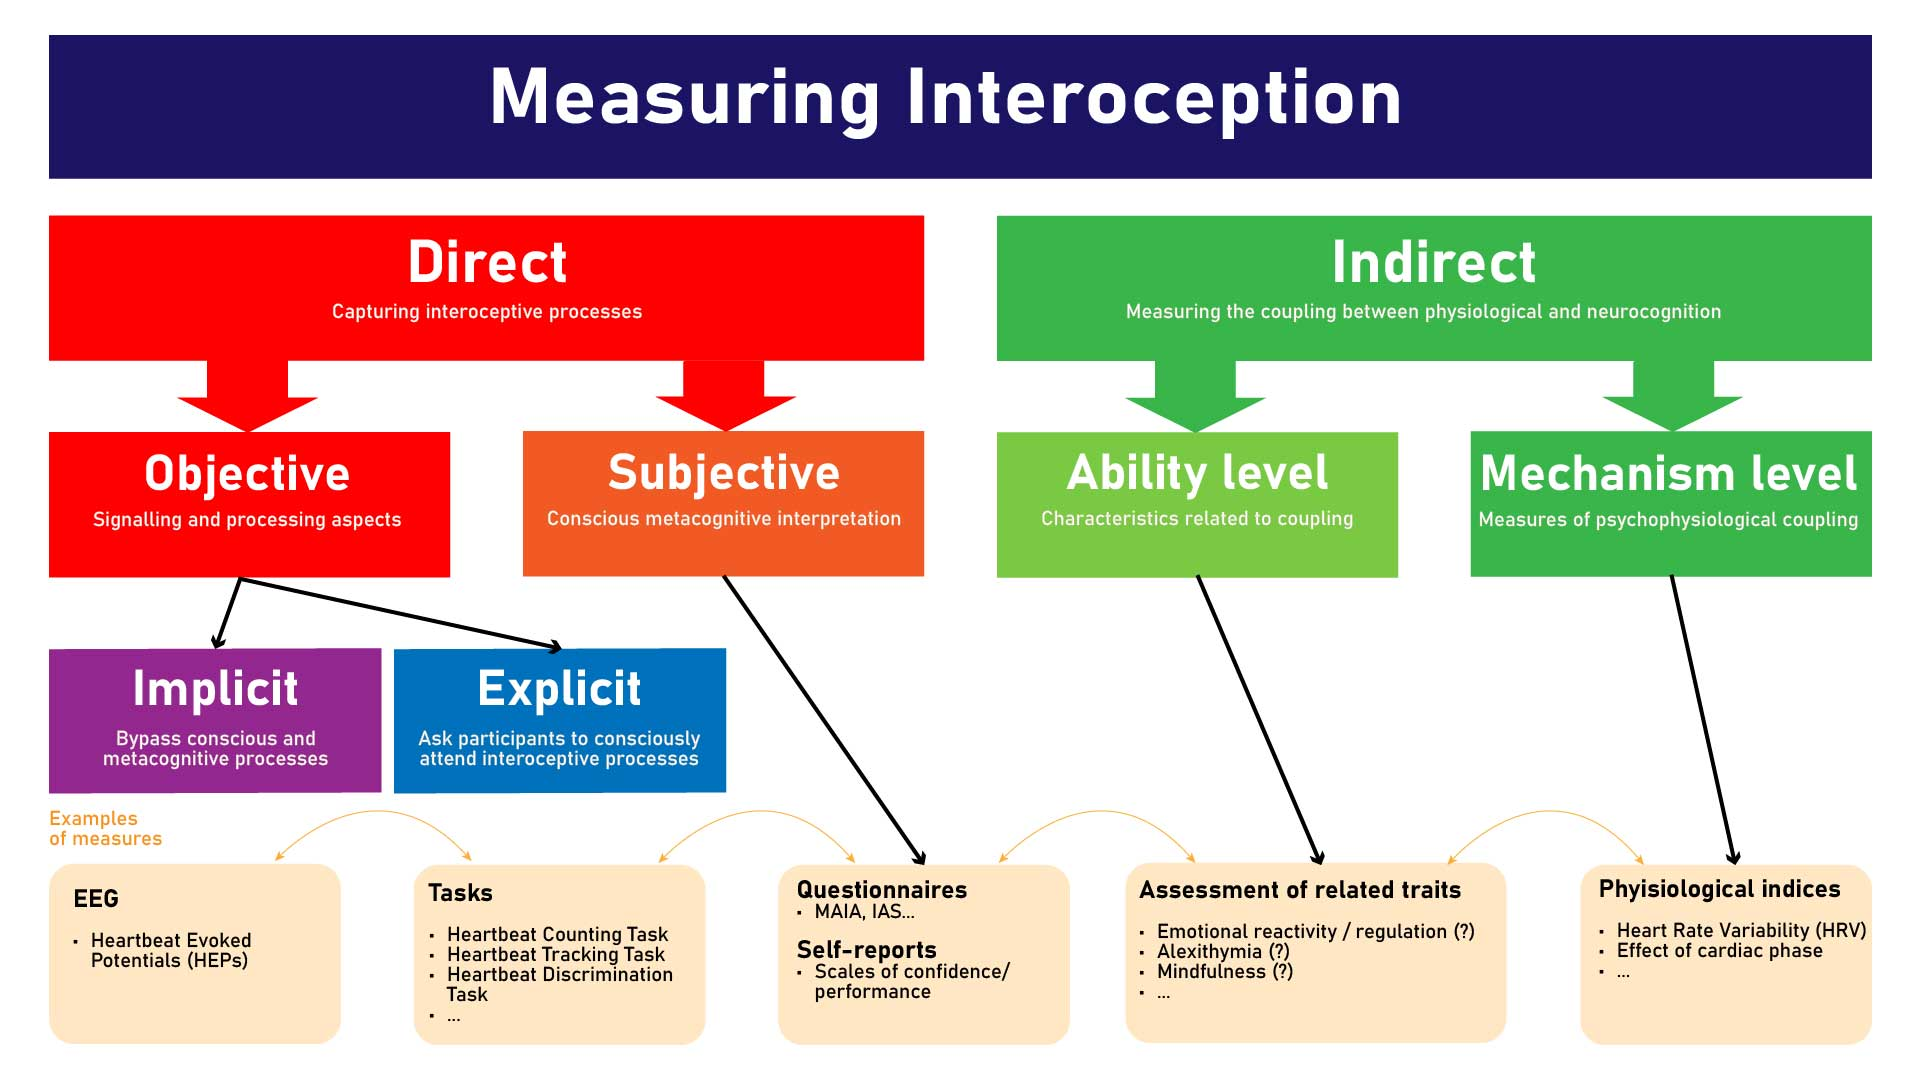
\includegraphics[width=6.4in,height=\textheight,keepaspectratio]{figures/MeasuringInteroception.jpg}

\end{figure*}

The use of subjective self-report questionnaires to measure deeply
embodied functions might seem paradoxical. However, recent redefinitions
of interoception emphasize the role of high-level and metacognitive
elaboration of interoceptive information. These redefinitions provide
theoretical grounding to support the idea that some facets of
interoception, including participants' metacognitive beliefs, can be
assessed subjectively (\citeproc{ref-khalsa2018interoception}{Khalsa,
Adolphs, Cameron, Critchley, Davenport, Feinstein, Feusner, Garfinkel,
Lane, Mehling, \& others, 2018};
\citeproc{ref-suksasilp2022towards}{Suksasilp \& Garfinkel, 2022}). This
approach offers useful and interesting measures
(\citeproc{ref-lin2023}{Lin et al., 2023};
\citeproc{ref-murphy2019}{Murphy et al., 2019}).

The notion that self-reports might not reflect the same processes as
other interoception measures is important to contextualize the apparent
lack of convergence between measures in the field
(\citeproc{ref-desmedt2022measures}{Desmedt et al., 2022}). While few
studies have explored the correlation between objective interoceptive
measures, such as the Heartbeat Counting Task (HCT,
\citeproc{ref-schandry1981heart}{Schandry, 1981}) and the Heartbeat
Detection Task (HDT, \citeproc{ref-kleckner2015methodological}{Kleckner
et al., 2015}), and correspondent self-report measures, existing
findings typically show weak or no correlations
(\citeproc{ref-brand2023}{Brand et al., 2023}; e.g., task-based accuracy
vs.~self-reported accuracy, \citeproc{ref-murphy2019}{Murphy et al.,
2019}).

Even among self-report measures low correlations have been observed,
suggesting that these measures, while group in the same umbrella term of
self-report assess different facets of interoception. A recent
systematic review by Desmedt et al.
(\citeproc{ref-desmedt2022measures}{2022}) examined whether various
questionnaires designed to assess ``interoceptive sensibility'' truly
measure the same construct. Notably, Garfinkel et al.
(\citeproc{ref-garfinkel2015knowing}{2015}) defines interoceptive
sensibility as the self-reported tendency to focus on and detect
internal sensations, whereas Khalsa, Adolphs, Cameron, Critchley,
Davenport, Feinstein, Feusner, Garfinkel, Lane, Mehling, and others
(\citeproc{ref-khalsa2018interoception}{2018}) defines it more narrowly,
excluding the ability to detect these signals. According to Desmedt et
al. (\citeproc{ref-desmedt2022measures}{2022}), most authors adopt the
latter definition. The review found that these questionnaires measure
related but distinct constructs, leading researchers to mistakenly
treating them as equivalent measures of interoceptive sensibility. A
better understanding of what is being measured with different
questionnaires and dimensions, as well as their potential overlaps with
other constructs (e.g., alexithymia, body awareness), is thus needed to
clarify the role of self-reports in the assessment of interoception.

A recently developed scale with a rapidly growing popularity is the
Interoceptive Accuracy Scale (IAS, \citeproc{ref-murphy2019}{Murphy et
al., 2019}). The IAS consists of 21 Likert-scale items that query how
accurately one can perceive different bodily signals, with one item per
physiological modality such as respiration (\emph{``I can always
accurately perceive when I am breathing fast''}), heart (e.g \emph{``I
can always accurately perceive when my heart is beating fast''}), skin
(e.g \emph{``I can always accurately perceive when something is going to
be ticklish''}), arousal or bodily functions like coughing (e.g
\emph{``I can always accurately perceive when I am going to cough''}) or
urinating (e.g.~\emph{``I can always accurately perceive when I need to
urinate''}). Interestingly, the IAS' statements are about specific
interoceptive behaviours, which is a notable difference with other
popular interoception questionnaires, such as the Multidimensional
Assessment of Interoceptive Awareness scale (MAIA,
\citeproc{ref-mehling2012}{Mehling et al., 2012}; MAIA-2,
\citeproc{ref-mehling2018multidimensional}{Mehling et al., 2018}), which
contains more general and metacognitive items (e.g., \emph{``I trust my
body sensations''}, \emph{``I can notice an unpleasant body sensation
without worrying about it''}).

Although the original validation study suggested a two-factor structure
for the IAS, the authors underline its acceptable but imperfect fit
(\citeproc{ref-murphy2019}{Murphy et al., 2019, p. 127}), calling on
further investigation of the scale's factor structure. Notably, the
authors did not define these factors, as no clear explanations were
evident. They suggested that the first factor reflects the perception of
interoceptive signals, while the second pertains to signals that may be
difficult to perceive solely through interoceptive information.

\textbf{note to dom}:Morin et al. (\citeproc{ref-morin2016}{2015}) is a
methodological paper on ESEM

Other follow-up studies using confirmatory factor analysis (CFA) and
structural modeling have identified different optimal solutions. Some
studies, like Brand et al. (\citeproc{ref-brand2023}{2023}), reported a
1-factor solution, while Lin et al. (\citeproc{ref-lin2023}{2023}) and
Campos et al. (\citeproc{ref-campos2021}{2021}) found bifactor solutions
- one general factor and a set of lower-level factors
(\citeproc{ref-rodriguez2016evaluating}{Rodriguez et al., 2016}) - to be
the best fit. Notably, the only other study to report a 2-factor
solution was conducted by Koike and Nomura
(\citeproc{ref-koike2023}{2023}), who performed an Exploratory Factor
Analysis (EFA) assuming 2 factors to align with the findings from the
original validation paper.

Discussions have also been focused on specific items. For instance,
Murphy et al. (\citeproc{ref-murphy2019}{2019}) notes that some items
might measure direct interoceptive signals such as cardioception, while
others might capture phenomena not perceivable through interoceptive
signals alone (e.g., ``bruising''; p.~119). Lin et al.
(\citeproc{ref-lin2023}{2023}) also highlights their correlation
analysis, showing five locally dependent pairs and three items (touch,
blood sugar, bruise) with exceptionally high difficulty and low
discrimination. Additionally, Campos et al.
(\citeproc{ref-campos2021}{2021}) reported ``tickle'' to be the only
item that reflected more specific factors than the general factor.
Interestingly, Lin et al. (\citeproc{ref-lin2023}{2023}) reported that
all items of the IAS grouped together using a new approach, Exploratory
Graph Analysis (EGA, \citeproc{ref-golino2017exploratory}{Golino \&
Epskamp, 2017}), to assess convergent and discriminant validity,
providing further evidence for unidimensionality.

The IAS has naturally been compared to other interoception-related
scales, and shows a positive correlations with most facets of the MAIA
(\citeproc{ref-mehling2018multidimensional}{Mehling et al., 2018}),
except for the Non-Distracting and Not-Worrying subscales
(\citeproc{ref-brand2023}{Brand et al., 2023}). Interestingly, findings
on the correlation between the IAS and the body awareness dimension of
the Body Perception Questionnaire (BPQ-A,
\citeproc{ref-porges1993body}{Porges, 1993}) have been mixed: some
studies report small positive correlations
(\citeproc{ref-brand2023}{Brand et al., 2023};
\citeproc{ref-campos2021}{Campos et al., 2021};
\citeproc{ref-koike2023}{Koike \& Nomura, 2023}), while others find
small negative correlations (\citeproc{ref-lin2023}{Lin et al., 2023})
or no correlation at all (\citeproc{ref-murphy2019}{Murphy et al.,
2019}). Small positive correlations have also been observed with the
``observation'' and ``description'' subscales of the Five Facet
Mindfulness Questionnaire (FFMQ, \citeproc{ref-baer2006using}{Baer et
al., 2006}; \citeproc{ref-brand2023}{Brand et al., 2023};
\citeproc{ref-koike2023}{Koike \& Nomura, 2023}), as well as with the
``non-reactivity'' and ``acting with awareness'' subscales
(\citeproc{ref-koike2023}{Koike \& Nomura, 2023}). Additionally, the IAS
has shown a positive correlation with the interoceptive awareness
subscale of the Eating Disorder Inventory (\citeproc{ref-lin2023}{Lin et
al., 2023}) and a negative correlation with the Interoceptive Confusion
Questionnaire (\citeproc{ref-brand2023}{Brand et al., 2023}; ICQ,
\citeproc{ref-brewer2016alexithymia}{Brewer et al., 2016};
\citeproc{ref-murphy2019}{Murphy et al., 2019}). Lastly, small positive
correlations have also been reported with the Interoceptive Attention
Scale (\citeproc{ref-koike2023}{Koike \& Nomura, 2023}; IATS,
\citeproc{ref-lin2023}{Lin et al., 2023}), though studies have also
found no correlation between these measures
(\citeproc{ref-gabriele2022dissociations}{Gabriele et al., 2022}).
Interestingly, the IAS and the IATS supposedly measure two different
interoceptive processes (i.e., accuracy and attention, respectively)
which contradict Murphy et al. (\citeproc{ref-murphy2019}{2019})
proposed 2x2 framework.

While assessing the validity of an interoception scale can be conceived
as theoretically challenging, several measures have been used to assess
convergent validity for the the IAS, including expected negative
associations with alexithymia (\citeproc{ref-brand2023}{Brand et al.,
2023}; \citeproc{ref-campos2021}{Campos et al., 2021};
\citeproc{ref-koike2023}{Koike \& Nomura, 2023};
\citeproc{ref-lin2023}{Lin et al., 2023};
\citeproc{ref-murphy2019}{Murphy et al., 2019}), somatic symptoms
(\citeproc{ref-brand2023}{Brand et al., 2023};
\citeproc{ref-koike2023}{Koike \& Nomura, 2023};
\citeproc{ref-lin2023}{Lin et al., 2023}), depressive symptoms
(\citeproc{ref-brand2023}{Brand et al., 2023};
\citeproc{ref-koike2023}{Koike \& Nomura, 2023};
\citeproc{ref-lin2023}{Lin et al., 2023}), anxiety
(\citeproc{ref-brand2023}{Brand et al., 2023}), neuroticism
(\citeproc{ref-brand2023}{Brand et al., 2023}) and self-esteem
(\citeproc{ref-murphy2019}{Murphy et al., 2019}).

The current study aims at 1) clarifying the structure of the IAS with a
meta-analytic approach that leverages existing data and contrast the
traditional CFA/SEM factor-based analyses with network-based ones such
as EGA; 2) the second part will provide an overview of the dispositional
correlates of the IAS, clarifying the pattern of associations which is
key to better understand the nature, place and role of interoception
questionnaires within a larger context.

\subsection{Study 1}\label{study-1}

The goal of study 1 is to re-analyse and assess the factor structure of
the IAS by taking advantage of the large number of open-access datasets
(\citeproc{ref-arslanova2022}{Arslanova et al., 2022};
\citeproc{ref-brand2022}{Brand et al., 2022};
\citeproc{ref-brand2023}{Brand et al., 2023};
\citeproc{ref-campos2021}{Campos et al., 2021};
\citeproc{ref-gaggero2021}{Gaggero et al., 2021};
\citeproc{ref-lin2023}{Lin et al., 2023};
\citeproc{ref-murphy2019}{Murphy et al., 2019};
\citeproc{ref-todd2022}{Todd et al., 2022}; \citeproc{ref-von2023}{Von
Mohr et al., 2023}). While combining these studies might provide a more
robust and generalizable understanding of the IAS' factor structure, we
also additionally provide an individual analysis (i.e., on all samples
separately) to add nuance to the general picture, as all studies differ
in their sample sizes, demographics, language, and procedure.

\subsubsection{Methods}\label{methods}

\paragraph{Datasets.}\label{datasets}

Our search focused on studies citing the original IAS validation paper
(\citeproc{ref-murphy2019}{Murphy et al., 2019}), identifying 136 papers
(as of 01/05/2024). To qualify for inclusion, papers needed to (1)
provide accessible data in open-access, (2) employ the IAS as a measure,
and (3) report individual IAS items scores. A total of 10 studies was
included (see \textbf{Table 1}). We also included the data of two
unpublished (but already open-access) studies from the authors and one
from another researcher. The total N participants was 32,214
participants (\emph{Mean} = 48.6 years, \emph{SD} = 13.1, 71.6\%
Female).

\begin{landscape}

\begin{table}
\fontsize{9.0pt}{10.8pt}\selectfont
\begin{tabular*}{\linewidth}{@{\extracolsep{\fill}}lllrrrrl}
\toprule
Sample & Subsample & Language & N & Age (Mean  ± SD) & Range & Female \% & Availability \\ 
\midrule\addlinespace[2.5pt]
Murphy et al., (2020) &  &  &  &  &  &  &  \\ 
 & Sample 1 & English & 451 & 25.8 ± 8.4 & 18-69 & 69.4\% &  \\ 
 & Sample 2 & English & 375 & 35.3 ± 16.9 & 18-91 & 70.1\% & https://osf.io/3m5nh \\ 
Gaggero et al., (2021) &  & English and Italian & 814 & 24.9 ± 5.3 & 18-58 & 60.3\% & https://osf.io/5x9sg \\ 
Campos et al., (2022) &  & Portuguese & 515 & 30.7 ± 10.5 & 18-72 & 59.6\% & https://osf.io/j6ef3 \\ 
Todd et al., (2022) &  & English & 802 & 48.6.6 ± 14.1* & 18-92* & 50\%* & https://osf.io/ms354 \\ 
Arslanova et al., (2022) &  & English & 143 & 28.5 ± 7.6 & 18-73 & 46.8\% & https://osf.io/mp3cy \\ 
Brand et al., (2022) &  & German & 619 & 43.9 ± 14.5 & 18-78 & 78.7\% & https://osf.io/xwz6g \\ 
Brand et al., (2023) &  &  &  &  &  &  &  \\ 
 & Sample 1 & German & 522 & 23.4 ± 6.7 & 18-79 & 79.5\% &  \\ 
 & Sample 2 & German & 1993 & 32.0 ± 12.6 & 16-81 & 77.7\% & https://osf.io/3f2h6 \\ 
 & Sample 3 & German & 802 & 27.3 ± 9.3 & 18-72 & 68.9\% &  \\ 
Lin et al., (2023) &  &  &  &  &  &  &  \\ 
 & Sample 1 & Chinese & 1166 & 32.5 ± 8.4 & 16-60 & 57.0\% &  \\ 
 & Sample 2 & Chinese & 500 & 37.4 ± 7.4 & 20-60 & 56.2\% & https://osf.io/3eztd \\ 
VonMohr et al., (2023) &  & English & 21843 & 56.5 ± 14.4 & 18-93 & 73.2\% & https://osf.io/7p9u5 \\ 
Makowski et al., (2023a) &  & English & 485 & 30.1 ± 10.1 & 18-73 & 50.3\% & https://github.com/RealityBending/IllusionGameReliability \\ 
Makowski et al., (2023b) &  & English & 836 & 25.1 ± 11.3 & 17-76 & 53.0\% & https://github.com/DominiqueMakowski/PHQ4R \\ 
Makowski et al., (2023c) &  & English & 104 & 21.6 ± 5.0 & 18-50 & 76\% & https://github.com/RealityBending/InteroceptionPrimals \\ 
Poreiro et al., (2024) &  & English & 107 & 26.8 ± 9.2 & 18-57 & 74.8\% & https://osf.io/49wbv \\ 
Poreiro et al., unpublished &  & English & 131 & 30.9 ± 12.0 & 18-60 & 75.9\% &  \\ 
Total &  &  & 32216 & 48.6 ± 13.1 & 17-93 & 71.6 &  \\ 
\bottomrule
\end{tabular*}
\begin{minipage}{\linewidth}
* Information taken from the sample description of relevant paper rather than recomputed.\\
\end{minipage}
\end{table}



\end{landscape}

\paragraph{Statistical Analysis.}\label{statistical-analysis}

To examine the factor structure of the IAS, a two-step approach was
employed. First, Exploratory Graph Analysis (EGA), was used to estimate
the dimensions via network estimation and community detection, alongside
assessing the stability of dimensions and items using the bootstrapping
techniques (\citeproc{ref-golino2017exploratory}{Golino \& Epskamp,
2017}). The selection of EGA was motivated by its capability to handle
complex, multidimensional data and provide robust dimension estimates. A
novel network psychometrics - Unique variable analysis (UVA,
\citeproc{ref-christensen2023unique}{Christensen et al., 2023}) -
approach based on the weighted topological overlap will be computed to
evaluate which items have substantial local dependence (\textgreater{}
0.25). Subsequently, exploratory factor analysis (EFA) was employed
followed by confirmatory factor analysis (CFA).

\subsubsection{Results}\label{results}

Visualizing the distribution of the items for all samples suggests the
presence of a consistent modal value (Figure~\ref{fig-distributions}).
In other words, participants are most likely to answer 4/5 (i.e., agree)
on most items (but ``affective touch'', ``blood sugar'', and ``bruise''
that exhibit a different distributional pattern). Additionally, one can
note the low density on extreme values (1 and 5), meaning that the bulk
of answers (i.e., 99\%) varies between 3 values. The interindividual
variability seems improved in the samples using an analogue scale,
displaying a more continuous and progressive spread of answers.

\begin{figure}

\caption{\label{fig-distributions}Distribution of responses for all
items across various datasets.}

\centering{

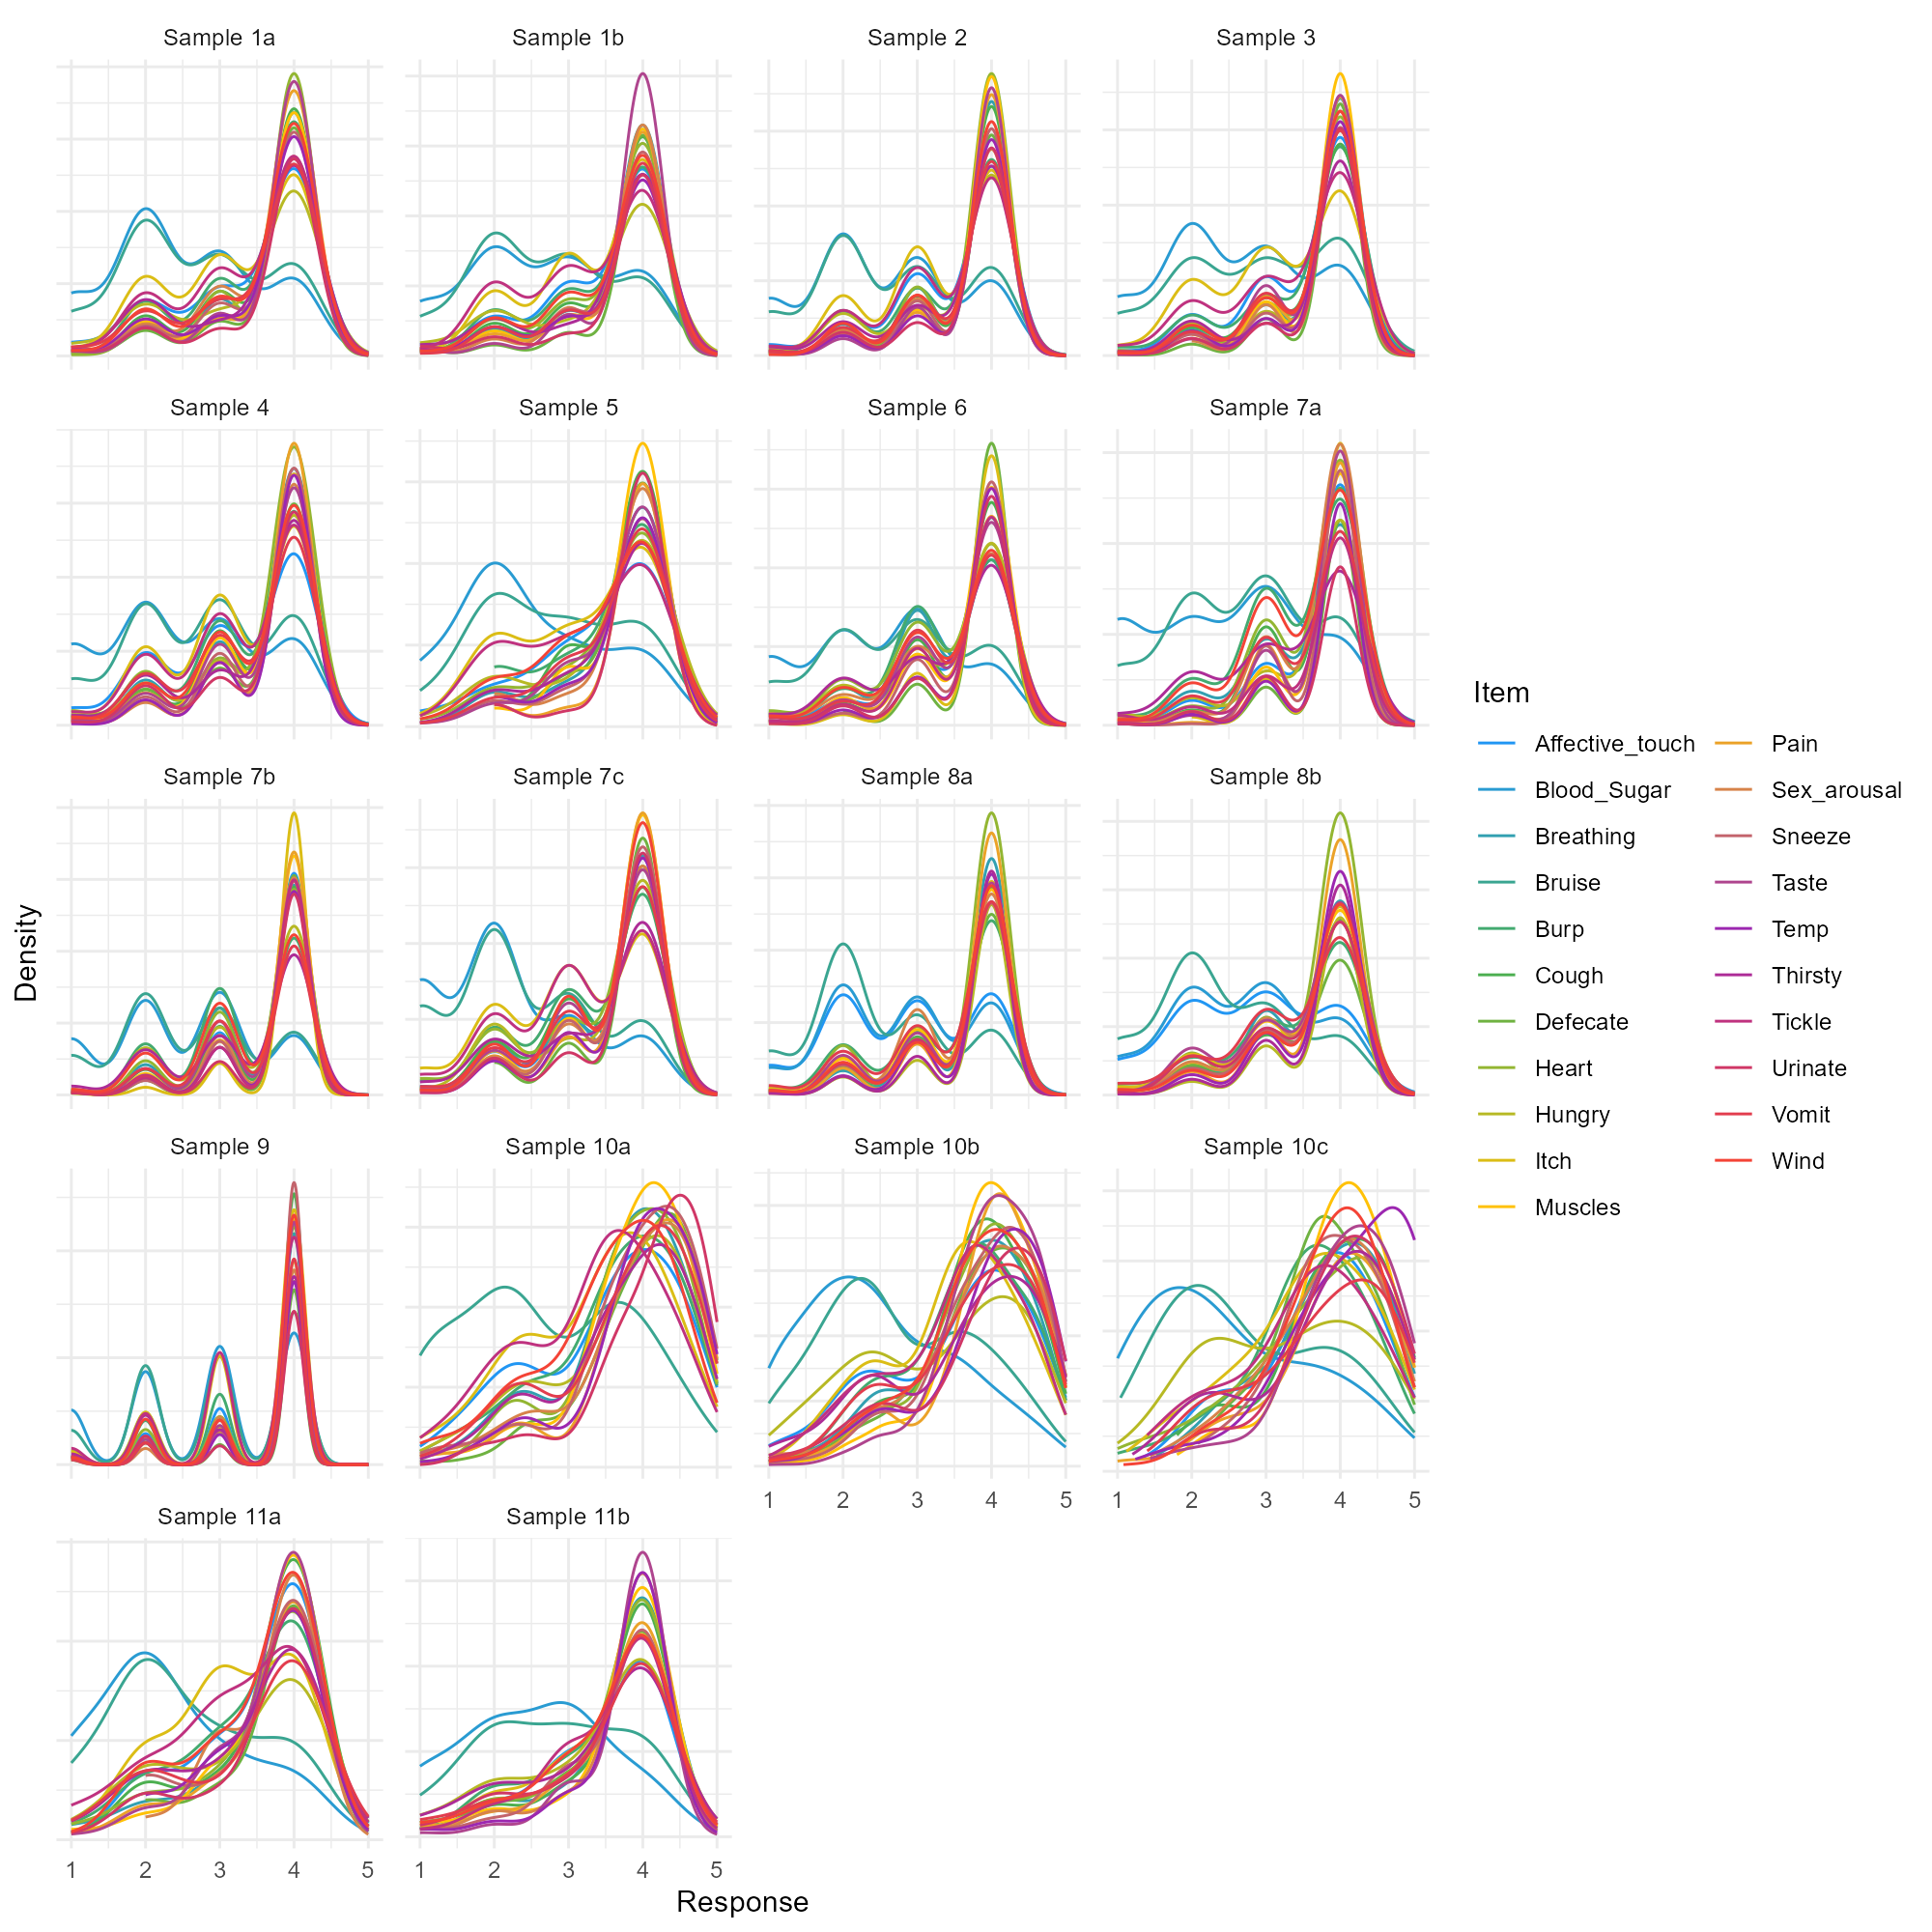
\includegraphics[width=6.67in,height=\textheight,keepaspectratio]{figures/Figure1.png}

}

\end{figure}%

\paragraph{Correlations.}\label{correlations}

The correlation analysis revealed that the items overall have positive
intercorrelation patterns with no clear structure emerging. This remains
the same across all samples. However, there are possibly some
higher-order groupings emerging for the 2 analog-scale samples.

\paragraph{EGA.}\label{ega}

The UVA revealed that there are two large to very large redundant
variables when taking all samples into account. Namely, ``itch'' and
``tickle'', where ``tickle'' should be removed, and ``itch'' should be
kept. There are several more items that are moderately to largely
redundant, namely, ``wind'' and ``burp'', and ``urinate'' and
``defecate''. On top of that, ``sneeze'' and ``cough'', ``heart'' and
``breathing'', and ``hungry'' and ``thirsty'' seem to have small to
moderate redundancy. These findings are rather consistent across the
samples with minor differences, such as that when the questionnaire had
an analog scale, there seems to be no large to very large redundant
items but ``itch'' and ``tickle'' remain moderately to largely redundant
and ``heart'' and ``breathing'' small to moderately redundant in one
sample.

According to the network analysis, using the Walktrap and Louvain
algorithms applied to Glasso networks, a 4-factor structure fits the
questionnaire best across all data sets. This is rather consistent
within the data sets, where some samples indicate 3-factor structure,
and some a 5-factor structure would fit well too. The 4-factor structure
model with the best fit entails the following items per group: 1) itch,
tickle, bruise, blood sugar; 2) burp, wind, cough, sneeze, vomit; 3)
affective touch, sexual arousal, muscles, temperature, pain, and taste;
4) Heart, breathing, hungry, thirsty, urinate, and defecate.

Stability analysis, employing 500 bootstrap iterations, also favoured
the 4-factor solution for its greater stability. Most items, except for
`affective touch,' demonstrated stability levels exceeding 0.90,
indicating structural consistency and reliability
(\citeproc{ref-christensen2021}{Christensen \& Golino, 2021}). These
findings underscore the robustness of the identified 4-dimensional
structure.

When accounting for all samples, the factor analysis reveals that a
4-factor structure fits best. The exploratory factor analysis revealed
that 4 latent factors (oblimin rotation) accounted for 41.58\% of the
total variance of the original data (MR1 = 14.45\%, MR3 = 11.76\%, MR2 =
8.09\%, MR4 = 7.28\%). Since UVA identified ``tickle'' as the item to be
removed---and it also had the lowest uniqueness value in factor analysis
with a similar loading to ``itch''---'' it was excluded from subsequent
analyses.

CFA was computed with the removal of the item ``tickle'' as it was
constantly flagged as redundant. This analysis compared 5 models: a
single-factor solution, a 4-factor solution, a 5-factor solution, a
6-factor solution and a 7-factor solution. The latter was preferred in
most datasets, including with indices that penalise increased number of
parameters (such as BIC). There was no evidence for higher order
factors.

\subsubsection{Discussion}\label{discussion}

In this study, several datasets were analyzed for a meta analysis of the
structure of the IAS. The findings reveal that a 4-factor model fits the
IAS best. Additionally, the lowest level structure (pairs of items) seem
to be the most robust, especially for samples using Likert scales (some
higher-order groupings might emerge for the 2 analog-scale samples).
There was no clear evidence for higher-order factors.

These findings contrast with previous research, which all found that
2-factor model (\citeproc{ref-koike2023}{Koike \& Nomura, 2023};
\citeproc{ref-murphy2019}{Murphy et al., 2019}), 1-factor model
(\citeproc{ref-brand2023}{Brand et al., 2023}) and bifactor model
(\citeproc{ref-campos2021}{Campos et al., 2021};
\citeproc{ref-lin2023}{Lin et al., 2023}) fits the data best. While this
analysis also revealed an okay fit for the 1-factor model, the 4-factor
model was superior. The 4-factor structure reveals different `hubs' of
items that are related, not only in this structure analysis, but also in
underlying mechanisms. The `wind-burp-cough-sneeze-vomit' category, for
example, only entails items that are linked to excretion through the
mouth. The other categories are organized similarly. This organization
and structure is useful for further analysis, as the data can be
analyzed and interpreted according to a grouping that is coherent in
result, as well as underlying mechanisms.

\textbf{note to dom}: what stats do you mean here? the UVA one?

There are several items that show redundancy suggesting that adapting
the IAS would be beneficial for validity. Based on the given results, we
suggest removing the tickle, while keeping the itch item
{[}\textbf{todo}: stats?{]}. Other items with slight redundancy were
``hungry'' and ``thirsty'', ``urinate'' and ``defecate'', and ``sneeze''
and ``cough''.

Interestingly, Lin et al. (\citeproc{ref-lin2023}{2023}) also found that
``tickle'' and ``itch'' were redundant, which led them to excludw one of
them. Although, the reason being that the character for both words is
the same in the Chinese language. On top of that, they came up with a
shortened version of the IAS, excluding further items, resulting in a
12-item IAS, which aligns with our findings, suggesting that further
items are ambiguous as to whether they should be removed. Their 12-item
IAS included the ``hunger'', ``breath'', ``urinate'', ``taste'',
``vomit'', ``cough'', ``temperature'', ``sexual arousa'', ``wind'',
``muscle'', ``pain'', ``itch'' items.\\
In contrast, other findings also found ``tickle'' to be redundant but
did not suggest excluding items (\citeproc{ref-campos2021}{Campos et
al., 2021}).

The findings indicate a high proportion of answers at 4 (see Figure 1),
especially when using a 5-step scale. The analogue scale shows a more
dispersed distribution, with some answers indicating the highest 5/5,
which was not the case in Likert-scales. Therefore, we recommend using
an analog scale for the IAS.

Before this paper, the IAS had not yet been used or analyzed with an
analog scale, rather than a five-step scale. Therefore, this study
provides a novel approach to improving the IAS in a simple manner.

\subsubsection{Limitations and Future
Directions}\label{limitations-and-future-directions}

There are several limitations to the IAS. There are some redundant
items, the 5-point scale does not provide great variability, and the
structure could be improved. Therefore, improving the IAS, or creating a
new questionnaire investigating interoception could be useful to
achieving reliable and accurate indication of interoceptive awareness.

\subsection{Study 2}\label{study-2}

Study 2 aims to investigate correlates of the IAS. Correlations of the
IAS will be computed to assess the relationship between subjective
interoceptive accuracy and other subjective measures of interoception,
mood, psychopathology, personality, and beliefs. Investigating
correlates will help validate the IAS, as well as other interoceptive
measures in the future.

\subsubsection{Methods}\label{methods-1}

\paragraph{Materials.}\label{materials}

The questionnaires used for the IAS correlates are listed in
\textbf{Table 2} (\textbf{TODO: add the rest of the questionnaires,
sample items and references}).

\begin{table}[t]
\fontsize{6.8pt}{8.1pt}\selectfont
\begin{tabular*}{\linewidth}{@{\extracolsep{\fill}}lrlrrl}
\toprule
Questionnaire & Number of Dimensions & Assessment & Number of Items & Scoring & Example Items \\ 
\midrule\addlinespace[2.5pt]
{\bfseries Interoceptive Related} &  &  &  &  &  \\ 
MAIA-2 & 8 & Interoceptive awareness & 37 & 6-point Likert scale & I notice when I am uncomfortable in my body \\ 
BPQ-SF & 2 & Body awareness and autonomic reactivity & 46 & 5-point Likert scale & My heart often beats irregularily \\ 
BPQ-VSF & 1 & Body awareness & 12 & 5-point Likert scale & My mouth being dry \\ 
ICQ & 3 & Interoceptive confusion & 20 & 5-point Likert scale &  I cannot tell when my muscles are sore or tight \\ 
TAS-20 & 3 & Alexithymia & 20 & 5-point Likert scale & I have feelings I can't quite identify \\ 
BVAQ & 5 & Alexithymia & 40 & 5-point Likert scale & I like to tell others how I feel \\ 
{\bfseries Mood} &  &  &  &  &  \\ 
BDI-II & 2 & Depressive symptoms severity & 21 & 4-point scale & I feel sad much of the time \\ 
PHQ-4 & 2 & Depression and Anxiety & 4 & 4-point Likert scale & Little interest or pleasure in doing things \\ 
PHQ-9 & 1 & Depressive symptoms & 9 & 4-point Likert scale & Feeling tired or having little energy? \\ 
PHQ-15 & 1 & Somatic symptom distress & 15 & 3-point scale & Over the last week, how often have you been bothered by back pain? \\ 
MFQ & 1 & Mood and affect & 13 & 3-point scale & I felt miserable or unhappy \\ 
STAI-T & 1 & Trait anxiety & 20 & 4-point Likert scale & I worry too much about something that really doesn't matter \\ 
GAD-7 & 1 & General anxiety disorder symptoms & 7 & 4-point Likert scale & Not being able to stop or control worrying \\ 
{\bfseries Personality} &  &  &  &  &  \\ 
NEO-FFI (neuroticism subscale) & 1 & Neuroticism & 12 & 5-point Likert scale & I often feel inferior to others \\ 
Mini IPIP6 & 6 & Personality traits & 24 & Visual analogue scales & Am the life of the party \\ 
BFI-S & 5 & Personality traits & 10 & 7-point Likert scale & I see myself as someone who ...is considerate and kind to almost everyone \\ 
{\bfseries Psychopathology} &  &  &  &  &  \\ 
PID-5-SFF & 5 & Maladaptive personality traits & 25 & 4-point Likert scale & Plenty of people are out to get me \\ 
SPQ-BR & 9 & Schizotypy & 32 & 5-point Likert scale & I am an odd, unusual person \\ 
MSI-BPD & 1 & Borderline personality disorder & 9 & Dichotomous (yes/no) & Have any of your closest relationships been troubled by a lot of arguments or repeated breakups? \\ 
ASQ - Short & 5 & Autistic traits & 28 & 4-point Likert scale & I find it difficult to work out people’s intentions \\ 
{\bfseries Beliefs and Misbeliefs} &  &  &  &  &  \\ 
GCBS & 5 & Conspiracy beliefs & 15 & 5-point Likert scale & Secret organizations communicate with extraterrestrials, but keep this fact from the public \\ 
PI-18 & 3 & Primal world beliefs & 18 & 5-point Likert scale & Nearly everything in the world is beautiful \\ 
LIE scale & 4 & Lying tendencies & 16 & Visual analogue scales & I am a good liar \\ 
\bottomrule
\end{tabular*}
\end{table}



\paragraph{Statistical analysis.}\label{statistical-analysis-1}

Correlations will be computed using the correlation package under a
Bayesian framework (\citeproc{ref-ben2020effectsize}{Ben-Shachar et al.,
2020}).

\subsubsection{Results}\label{results-1}

\subsection{Average correlations}\label{average-correlations}

The EGA components captured grouping of items such as `wind' and `burp,
'cough' and `sneeze', `muscle' and `pain'. These groupings were used in
correlational analysis to analyse how much each pairing is associated
with other factor such as Alexithymia and with Mood disorders (see
figure 2).

\textbf{note}compute internal consistency

\paragraph{Correlations with body
measures.}\label{correlations-with-body-measures}

Alexithymia was assessed in the samples with the Bermond--Vorst
Alexithymia Questionnaire {[}BVAQ; Vorst and Bermond
(\citeproc{ref-vorst2001validity}{2001}){]} and the Toronto Alexithymia
Scale{[}TAS; Bagby et al. (\citeproc{ref-bagby1994twenty}{1994}){]}.

The BVAQ consists of 5 subscales - fantasising, idenitying, analysing;
verbalising and emotionalising - assessed with 40 items on a 5-point
Likert scale, from `defnitely applies to me' to `in no way applies to
me'. Additionally, the BVAQ reduces these subscales into two high order
factors, an affective component and a cognitive one, with high scores
being indicative of high proneness to alexithymia.

On average, the cognitive component of the BVAQ was weakly and
negatively correlated with all IAS pairs of items with the biggest
correlation being with the Itch/Bruise pair (r = -0.112) and the lowest
correlation beeing with the Muscle/Pain pair (r = -0.244). The affective
component of the BVAQ was positively, but very weak, correlated with all
pairs, with the biggest correlation being with the Itch/Bruise pair (r =
0.107). The only exception was a negative correlation with the
Urinate/Defecate pair (r = -0.036).

The TAS contains 20-items rated on a 5-point forced scale, from
`strongly disagree' to `strongly afree', divided into 3 dimensions -
difficulty identiying feelings, difficulty describing feelings, and
externally thinking. High scores on this scale also reflect higher
alexithymia.

All the three dimensions assessed with the TAS were on average
negatively correlated with all pairs of IAS items. The difficulty
describing feelings had its strongest correlation with Hungry/Thirsty (r
= -0.179) and weakest with the Wind/Burp (r = -0.117). while, the
difficulty describing feelings had its strongest correlation with
Muscle/Pain (r = -0.247) and weakest with Itch/Bruise (r = -0.157).
Lastly, the external thinking dimension was more correlated with the
Cough/Sneeze pair (r = -0.138) and less correlated with the
Hungry/Thirsty (r = -0.018).

The studies within our sample used the Body Perception Questionnaire
short-form (BPQ-SF) and the very-short form (BPQ-VSF) to assess
interoception (\citeproc{ref-cabrera2018assessing}{Cabrera et al.,
2018}). The BPQ-SF comprised of 46 items on a 5-point Likert scale
assessing body awareness (26 items) and autonomic reactivity (21 items).
The BPQ-VSF comprises of 12 items from the body awareness subscale of
the BPQ-SF. In this study, all scores assessing these two dimensions
were grouped together, hence no disitintion is made between awareness
measured with the BPQ-SF and the BPQ-VSF, or eith scores obtained only
using the awareness subscale.

\textbf{note to add:} discuss later

In general, all pairs of the IAS were positively,and weakily, associated
with the body awareness subscales, while negative and weakily correlated
with the autonomic reactivity subscale. The strongest correlation
identified between the IAS pairs and the body awereness subscale was
with the\\
Heart/Breathing pair (r = 0.151) whilst the strongest correlation with
the autonomic reactivity was with the Urinate/Defecate pair (r =
-0.235). The weakest correlation between the body awareness and the IAS
was with the Hungry/Thirsty pair (r = 0.055) and between the autonomic
reactivity and the IAS was with the Heart/Breathing pair (r = -0.106).

The MAIA was one of the most commonly used measures of interoception in
our study, with nine samples reporting its use. This 37-item
questionnaire assesses eight state-trait dimensions of interoception:
Noticing, Not-Distracting, Not-Worrying, Attention Regulation, Emotional
Awareness, Self-Regulation, Body Listening, and Trust. Responses are
rated on a scale from 0 (Never) to 5 (Always).

On average, all MAIA dimensions were positively and weakly to moderately
correlated with IAS pairings. Notably, the strongest correlations were
observed between the Noticing dimension and the Heart/Breathing pairing
(r = 0.394), Trusting and Hungry/Thirsty (r = 0.347), and Attention
Regulation and Heart/Breathing (r = 0.334). The Not-Distracting and
Not-Worrying subscales were generally positively correlated with IAS
pairings, with a few exceptions: Not-Distracting showed minimal
correlation with Cough/Sneeze (r = 0.0206) and Heart/Breathing (r =
-0.007), while Not-Worrying had a low correlation with Itch/Bruise (r =
0.031).

The Interoceptive Confusion Questionnaire (ICQ; Brewer et al.
(\citeproc{ref-brewer2016alexithymia}{2016})) was used to assess
individuals' difficulties in interpreting non-affective physiological
states, such as pain and hunger. The ICQ consists of 20 items rated on a
scale from 1 (``Does not describe me'') to 5 (``Describes me very
well''), with higher scores indicating greater interoceptive confusion.

The ICQ showed weak to moderate negative correlations with all IAS
pairings. The strongest correlation was observed with the Hunger/Thirsty
pairing (r = 0.348), while the weakest was with the Itch/Bruise pairing
(r = 0.207).

\paragraph{Correlations with mood
measures.}\label{correlations-with-mood-measures}

Mood disorders were assessed using several standardized measures,
including the General Anxiety Disorder-2 {[}GAD-2; Kroenke et al.
(\citeproc{ref-kroenke2007anxiety}{2007}){]}, the State-Trait Anxiety
Inventory {[}STAI; Spielberger
(\citeproc{ref-spielberger1970manual}{1970}){]} and its shorter version,
the STAI-5 (\citeproc{ref-zsido2020development}{Zsido et al., 2020}),
Beck's Depression Inventory {[}BDI; Beck et al.
(\citeproc{ref-beck1996beck}{1996}){]}, and the Mood and Feelings
Questionnaire {[}MFQ; Messer et al.
(\citeproc{ref-messer1995development}{1995}){]}. Additionally, the
Patient Health Questionnaire (PHQ) was administered in its 2-item
{[}PHQ-2; Kroenke et al. (\citeproc{ref-kroenke2003patient}{2003}){]},
9-item {[}PHQ-9; Kroenke et al.
(\citeproc{ref-kroenke2001phq}{2001}){]}, and 15-item {[}PHQ-15; Kroenke
et al. (\citeproc{ref-kroenke2002phq}{2002}){]} versions. Finally,
borderline personality traits were assessed using the McLean Screening
Instrument for Borderline Personality Disorder {[}MSI-BPD; Zanarini
(\citeproc{ref-zanarini2003zanarini}{2003}){]}.

The GAD-2, a brief screening tool for generalized anxiety disorder,
consists of two items rated on a scale from 0 (not at all) to 3 (nearly
every day). The STAI, a 40-item questionnaire rated on a 4-point Likert
scale (0 to 3), measures both state and trait anxiety. However, in our
study, most participants primarily completed the trait anxiety subscale.
In some samples, a shorter 5-item version (STAI-5) was used to assess
both state and trait anxiety.

On average, anxiety measures showed weak negative correlations with all
IAS pairs. Notably, the strongest correlations between the IAS pairings
and the GAD-2, STAI-T and STAIT-5 were observed with the Hungry/Thirsty
pair (r = -0.168, r = -0.270 and r = -0.248, respectively).

The BDI consists of 21 items measuring the severity of depressive
symptoms on a scale from 0 to 3. The total score is calculated by
summing the highest responses, which are then compared to six depression
severity levels, ranging from 1--10 (normal fluctuations in mood) to
over 40 (extreme depression). The PHQ-2 includes two items assessing the
frequency of depressive symptoms and anhedonia. The PHQ-2 is derived
from the PHQ-9, a nine-item screening tool used to assess depression
severity and monitor treatment response. Both questionnaires are
measured on on a scale from 0 (not at all) to 3 (nearly every day)

Depression measures showed weak to moderate negative correlations with
IAS pairings. The BDI (r = -0.372), PHQ-2 (r = -0.148), and PHQ-9 (r =
-0.241) correlated most with the Hungry/Thirsty pair, while the MFQ
correlated most with Heart/Breathing (r = -0.345) pair.

The PHQ-15 is a 15-item questionnaire that assesses somatic symptoms on
a 3-point scale (e.g., back pain). It exhibited its strongest
correlation with the Hungry/Thirsty pair (r = -0.241) and, on average,
showed weak negative correlations with all other IAS pairings.

Lastly, the MSI-BPD is a 10-item questionnaire used to assess
personality disorder, where items are rated on a dichotomous scale of 1
(present) and 0 (absent). The MSI-BPD also showed its strongest negative
correlation with the Hungry/Thirsty pair (r = -0.140) and was negatively
correlated with all other pairings, except for Cough/Sneeze, which
showed a slight positive correlation (r = 0.0219).

\paragraph{Correlations with psychopathology
measures.}\label{correlations-with-psychopathology-measures}

Maladaptive personality traits were assessed using the Personality
Inventory for DSM-5 Short Form {[}PID-5-SF; Thimm et al.
(\citeproc{ref-thimm2016personality}{2016}){]}, which measures five
domains: disinhibition, antagonism, detachment, negative affect, and
psychoticism. The scale consists of 25 items rated on a 4-point Likert
scale, ranging from 0 (very false or often false) to 3 (very true or
often true).

On average, all maladaptive personality traits assessed by the PID-5-SF
were weakly and negatively correlated with IAS pairings. The strongest
correlation was observed between the psychoticism dimension and the
Muscle/Pain pairing (r = -0.173).

Schizotypy was assessed using the Schizotypal Personality Questionnaire
-- Brief Revised Updated (SPQ-BRU; Davidson et al.
(\citeproc{ref-davidson2016schizotypal}{2016})), which consists of 32
items rated on a 5-point Likert scale ranging from strongly agree to
strongly disagree. This questionnaire evaluates four primary dimensions:
cognitive-perceptual (positive), interpersonal (negative), disorganized,
and social anxiety. These dimensions are further divided into nine
secondary factors: constricted affect, eccentricity, magical thinking,
lack of close friends, odd speech, referential thinking, social anxiety,
suspiciousness, and unusual perceptions.

On average, all nine factors were weakly and negatively correlated with
IAS pairings, with correlations ranging from r = -0.170 (between lack of
close friends and Muscles/Pain) to r = 0.102 (between magical thinking
and Itch/Bruise).

The short version of the Autism-Spectrum Quotient (ASQ-Short; Hoekstra
et al., 2011) was used to assess five autistic traits: social skills,
adherence to routines, cognitive flexibility (switching), imagination,
and patterns/numbers. The questionnaire consists of 28 items rated on a
4-point Likert scale, ranging from 1 (definitely agree) to 4 (definitely
disagree).

Overall, all pairings were weakly and negatively correlated with the ASQ
dimensions, except for the Itch/Bruise and Heart/Breathing pairings,
which showed weak positive correlations with the patterns/numbers trait
(r = 0.184 and r = 0.038, respectively). The strongest correlation was
observed between the imagination trait and the Wind/Burp pairing (r =
-0.218).

\paragraph{Correlations with personality
measures.}\label{correlations-with-personality-measures}

The Big Five Inventory-Short Form {[}BFI-S; Lang et al.
(\citeproc{ref-lang2011short}{2011}){]} and the Mini International
Personality Item Pool {[}Mini-IPIP6; Sibley et al.
(\citeproc{ref-sibley2011mini}{2011}){]} were used to assess general
personality traits. The BFI-S consists of 15 items rated on a 7-point
Likert scale, ranging from 1 (strongly disagree) to 7 (strongly agree),
measuring five personality factors: Openness, Conscientiousness,
Extraversion, Agreeableness, and Neuroticism. The Mini-IPIP6 assesses
six personality traits---Extraversion, Agreeableness, Conscientiousness,
Neuroticism, Openness, and Honesty-Humility---using 24 items. While this
questionnaire is typically scored on a 7-point Likert scale from 1 (very
inaccurate) to 7 (very accurate), an analogous scale was used in the
respective sample. Lastly, the Neuroticism subscale of the NEO
Five-Factor Inventory {[}Neo-FFI; Costa and McCrae
(\citeproc{ref-costa1992normal}{1992}){]} was used to assess
Neuroticism, consisting of 12 items rated on a 5-point Likert scale from
1 (strongly disagree) to 5 (strongly agree).

To assess correlations with the IAS pairings, scores were grouped across
personality dimensions due to the overlap among these traits (with the
exception of Honesty-Humility). On average, IAS pairings were positively
associated with most personality dimensions, though these correlations
were generally weak. The strongest correlation was observed between
Conscientiousness and the Hungry/Thirsty pairing (r = 0.164). Both
Honesty-Humility and Neuroticism were weakly and negatively correlated
with the IAS pairings, with the highest correlations observed for the
Hungry/Thirsty pairing (r = -0.217 and r = -0.200, respectively).

\paragraph{Correlations with other
measures.}\label{correlations-with-other-measures}

The IAS was also correlated with primal world beliefs, as measured by
the Primal Inventory {[}PI-18; J. D. Clifton and Yaden
(\citeproc{ref-clifton2021brief}{2021}){]}, which assesses beliefs about
the world being alive, good, safe, and enticing. Items that evaluate
neutral beliefs about the hierarchical order of importance in the world
(i.e., hierarchical), as well as beliefs about the comprehensibility of
most things and situations (i.e., understandable), and the belief that
the world is characterized by flux (i.e., changing) were added as well.
The scale contains 18 items ranging from 5 (Strongly agree) to 0
(strongly disagree).

Overall, most primal beliefs show weak positive correlations with all
pairings of the IAS. The strongest correlation is between the
hierarchical belief and the Hungry/Thirsty pairing (r = 0.181). Some
beliefs, however, exhibit negative correlations with certain pairings.
These negative correlations range from r = -0.0940 between the changing
belief and the Hungry/Thirsty pairing, to r = -0.00490 between the
Enticing belief and the Itch/Bruise pairing.

The Generic Conspiracist Beliefs Scale {[}GCBS; Brotherton et al.
(\citeproc{ref-brotherton2013measuring}{2013}){]} was used to assess
five facets of conspiracy beliefs: Extraterrestrial, Global
Conspiracies, Government Malfeasance, Information Control, and Personal
Wellbeing. The scale comprises 15 items rated on a 5-point Likert scale,
ranging from definitely not true (1) to definitely true (5).

Overall, the GCBS showed a weak but positive correlation with all facets
of the IAS, with the strongest correlation observed between Global
Conspiracies and Hungry/Thirsty (r = 0.140). Negative correlations were
found within the Global Conspiracies, Extraterrestrial, and Information
Control facets, though these were small, ranging from r = -0.0101 to r =
-0.0167.

Lastly, the Lying Profile Questionnaire {[}LIE; Makowski, Pham, et al.
(\citeproc{ref-makowski2023structure}{2023}){]} a 16 item visual analog
scale was used to assess 4 dispositional lying simensions: ability;
negativity, contextuality, and frequency.

Overall, most lying profile dimensions show weak correlations with IAS
pairings. Ability exhibits primarily weak positive correlations, with
the strongest observed for Wind/Burp (r = 0.082). In contrast, Frequency
tends to show weak negative correlations, ranging from Wind/Burp (r =
-0.062) to Muscles/Pain (r = -0.088). Contextuality displays mixed
correlations, with Itch/Bruise showing the strongest negative
association (r = -0.127), while Urinate/Defecate has a small positive
correlation (r = 0.045). Finally, Negativity is consistently positively
correlated with all pairings, with the strongest relationship found for
Hungry/Thirsty (r = 0.090).

\begin{figure}[H]

\caption{\textbf{Figure 2.} Correlates of the IAS}

{\centering 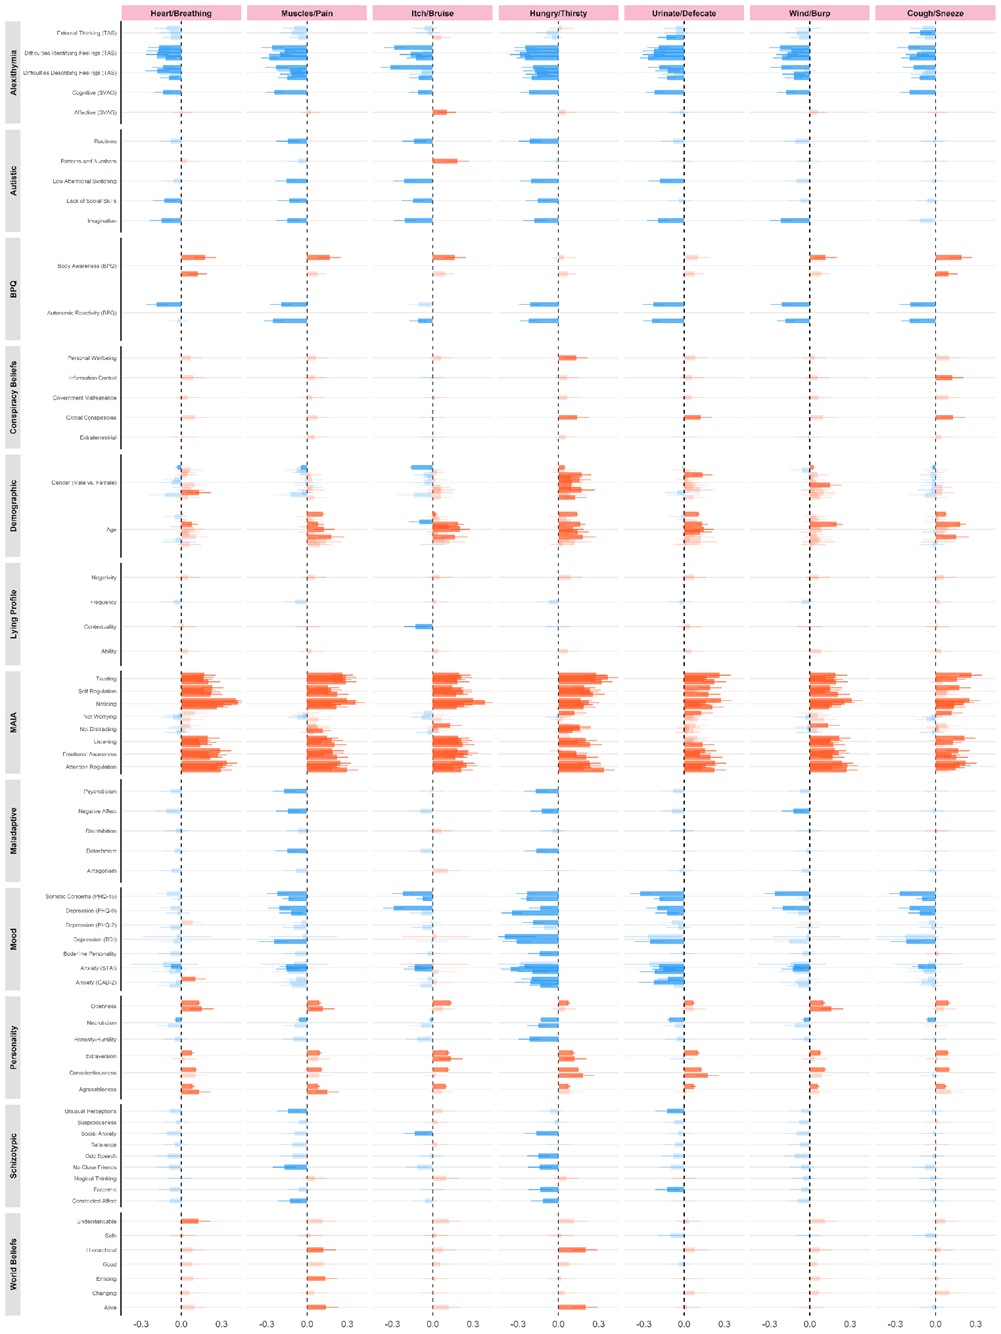
\includegraphics[width=9.48958in,height=\textheight,keepaspectratio]{figures/clipboard-1619164537.png}

}

\end{figure}%

\subsubsection{Discussion}\label{discussion-1}

Our findings confirm that interoception exists within a complex network
of correlates. Among these, alexithymia exhibits the strongest negative
correlation with the IAS, whereas the MAIA questionnaire shows the
strongest positive correlation. These correlates not only help explain
different aspects of interoception but also serve as valuable tools for
validating interoceptive measures.

While our results reveal various correlations with the IAS, they are
limited to the scope of the given questionnaire. Nonetheless, they
provide valuable insights into how interoception may relate to different
psychological and personality traits. The results show a consistent
pattern of correlations with other measures and highlight interesting
exploratory results, such as correlations between primal world beliefs
with the IAS.

Our analysis found a strong negative correlation between alexithymia and
IAS scores, aligning with previous research
(\citeproc{ref-brand2023}{Brand et al., 2023};
\citeproc{ref-herbert2011}{Herbert et al., 2011};
\citeproc{ref-murphy2019}{Murphy et al., 2019}). Similarly, a negative
correlation between autism and interoceptive awareness was observed in
our sample, consistent with prior findings
(\citeproc{ref-dubois2016}{DuBois et al., 2016}).

Conspiracy beliefs did not strongly correlate with IAS scores, though a
slight positive correlation was present. To our knowledge, this
relationship has not been previously explored. However, prior studies
have suggested connections between interoception and (political)
beliefs, potentially pointing to shared underlying mechanisms
(\citeproc{ref-ruisch2022}{Ruisch et al., 2022a}).

The relationship between interoception and lying profiles was also weak.
This contrasts with previous research suggesting associations between
interoception and deception (\citeproc{ref-makowski2023a}{Makowski, Lau,
et al., 2023}), warranting further investigation.

Mood and IAS scores exhibited a strong negative correlation, consistent
with prior studies that have documented similar findings
(\citeproc{ref-solanoluxf3pez2018}{Solano López \& Moore, 2018}).
Additionally, personality traits correlated with interoceptive accuracy
scores, reinforcing existing research linking personality and
interoception (\citeproc{ref-erle2021}{Erle et al., 2021}).

We also observed negative correlations between schizotypy and
interoception, in line with previous studies that identified a similar
relationship with interoceptive awareness, particularly in individuals
at risk for psychosis (\citeproc{ref-torregrossa2022}{Torregrossa et
al., 2022}).

Interestingly, world beliefs demonstrated significant positive
correlations with interoception. While this relationship has not been
previously documented, other forms of belief, such as political
ideology, have been linked to interoception
(\citeproc{ref-ruisch2022a}{Ruisch et al., 2022b}). Further research is
needed to determine whether world beliefs, which shape our perception of
reality (\citeproc{ref-clifton2020}{J. D. W. Clifton, 2020}), are
meaningfully connected to interoception.

Overall, our findings highlight the broad relevance of interoception
across various cognitive and affective traits, underscoring its
significance in both research and clinical contexts. By identifying
numerous correlates of the IAS, we contribute not only to a deeper
understanding of interoception's role in daily life but also to the
ongoing validation of the IAS and other interoceptive measures. This
analysis lays an important foundation for the development of new
interoceptive assessment tools, further advancing our comprehension of
interoception and its impact on human experience.

\subsection{General Discussion}\label{general-discussion}

Our analyses revealed that the IAS follows a four-factor structure with
an uneven distribution. While the findings indicate that the IAS
measures interoception adequately, there is room for improvement.
Additionally, different correlation measures with the IAS suggest
opportunities for further exploration of how interoception is assessed.
In the following section, we discuss the strengths and shortcomings of
the IAS, followed by proposed steps to enhance interoception
measurement.

Overall, the IAS is straightforward in its sensation-centered items.
However, several areas for improvement emerge from this study. Firstly,
redundant items should be removed, such as the ``itch'' item, as
highlighted in our analysis. Previous research also suggests redundancy
between itch and tickle items Campos et al.
(\citeproc{ref-campos2021}{2021}). Interestingly, while Campos et al.
(\citeproc{ref-campos2021}{2021}) does not recommend the removal of
either, Lin et al. (\citeproc{ref-lin2023}{2023}) argues for removing
the itch item due to their overlapping character representation.

Furthermore, this study recommends using analog scales instead of
5-point scales. The limited variability of the 5-point scale often
results in most responses clustering around 3 or 4. As shown in
Figure~\ref{fig-distributions}, adopting an analog scale significantly
increases variability. However, even with an analog scale, IAS
variability remains constrained. Greater variability allows for better
differentiation among participants, making dispersion an essential
factor for obtaining meaningful results. Enhancing variability would
therefore be beneficial for the IAS.

Despite these improvements, certain limitations persist in the IAS that
affect its accuracy. Notably, some modalities are underrepresented---for
instance, heart perception is measured by only one item. Expanding
modality coverage would enhance variability within each category,
leading to more nuanced results. Moreover, the IAS lacks a clear
theoretical or empirical structure, with only small item groupings.
Ideally, a scale should allow for clear groupings that support
meaningful data analysis. In this study, each group contained only two
items, resulting in low scores and limited variability. Additionally,
some IAS items are ambiguous, with their interpretation depending on
context. For example, an item about perceiving heartbeats and another
about vomiting could both relate to anxiety, leading to results that may
differ from initial expectations. Thus, the grouping and structure of
the IAS require refinement.

Another concern is that all IAS items are phrased positively, which may
influence participant responses. While positive phrasing has advantages,
it can also introduce response bias, leading to unidimensional results.
A more balanced phrasing approach, incorporating both positively and
negatively framed items, could yield more accurate responses.

Given these considerations, it is clear that context-specific,
cross-modal items---such as integrating cardioception and
respiroception---are needed. Recognizing the necessity for a refined
interoception scale, this study proposes the development of the
Multidimensional Interoceptive Inventory (MInt). This new scale will be
designed to align with recent findings on the IAS and interoception
research while allowing for direct comparison with IAS correlates.

{[}\textbf{TO DO}: add - previous work suggests the importance of
physiological contexts (Vlemincx et al., 2021){]} \textbf{I would rather
put that in the discussion in the suggestions for better scales}

\subsection{Conclusion}\label{conclusion}

The IAS is a valuable tool for measuring interoception compared to
existing questionnaires and methods. However, refining or even
redesigning the questionnaire could lead to a more precise and
comprehensive assessment. This study highlights the need for a new
interoception scale to advance research in the field. By identifying
various correlates of the IAS, this work paves the way for future
investigations into optimal interoceptive measures, ultimately laying
the foundation for the development of a more effective interoception
survey.

\subsection{References}\label{references}

\phantomsection\label{refs}
\begin{CSLReferences}{1}{0}
\bibitem[\citeproctext]{ref-arslanova2022}
Arslanova, I., Galvez-Pol, A., Kilner, J., Finotti, G., \& Tsakiris, M.
(2022). Seeing through each other's hearts: Inferring others' heart rate
as a function of own heart rate perception and perceived social
intelligence. \emph{Affective Science}, \emph{3}(4), 862--877.

\bibitem[\citeproctext]{ref-baer2006using}
Baer, R. A., Smith, G. T., Hopkins, J., Krietemeyer, J., \& Toney, L.
(2006). Using self-report assessment methods to explore facets of
mindfulness. \emph{Assessment}, \emph{13}(1), 27--45.

\bibitem[\citeproctext]{ref-bagby1994twenty}
Bagby, R. M., Parker, J. D., \& Taylor, G. J. (1994). The twenty-item
toronto alexithymia scale---i. Item selection and cross-validation of
the factor structure. \emph{Journal of Psychosomatic Research},
\emph{38}(1), 23--32.

\bibitem[\citeproctext]{ref-beck1996beck}
Beck, A. T., Steer, R. A., \& Brown, G. (1996). Beck depression
inventory--II. \emph{Psychological Assessment}.

\bibitem[\citeproctext]{ref-ben2020effectsize}
Ben-Shachar, M. S., Lüdecke, D., \& Makowski, D. (2020). Effectsize:
Estimation of effect size indices and standardized parameters.
\emph{Journal of Open Source Software}, \emph{5}(56), 2815.

\bibitem[\citeproctext]{ref-brand2023}
Brand, S., Meis, A. C., Tünte, M. R., Murphy, J., Woller, J. P.,
Jungmann, S. M., Witthöft, M., Hoehl, S., Weymar, M., Hermann, C., \&
Ventura-Bort, C. (2023). A multi-site German validation of the
Interoceptive Accuracy Scale and its relation to psychopathological
symptom burden. \emph{Communications Psychology}, \emph{1}(1).
\url{https://doi.org/10.1038/s44271-023-00016-x}

\bibitem[\citeproctext]{ref-brand2022}
Brand, S., Petzke, T. M., \& Witthöft, M. (2022). The differential
relationship between self-reported interoceptive accuracy and attention
with psychopathology. \emph{Zeitschrift f{ü}r Klinische Psychologie Und
Psychotherapie}.

\bibitem[\citeproctext]{ref-brewer2016alexithymia}
Brewer, R., Cook, R., \& Bird, G. (2016). Alexithymia: A general deficit
of interoception. \emph{Royal Society Open Science}, \emph{3}(10),
150664.

\bibitem[\citeproctext]{ref-brotherton2013measuring}
Brotherton, R., French, C. C., \& Pickering, A. D. (2013). Measuring
belief in conspiracy theories: The generic conspiracist beliefs scale.
\emph{Frontiers in Psychology}, \emph{4}, 279.

\bibitem[\citeproctext]{ref-cabrera2018assessing}
Cabrera, A., Kolacz, J., Pailhez, G., Bulbena-Cabre, A., Bulbena, A., \&
Porges, S. W. (2018). Assessing body awareness and autonomic reactivity:
Factor structure and psychometric properties of the body perception
questionnaire-short form (BPQ-SF). \emph{International Journal of
Methods in Psychiatric Research}, \emph{27}(2), e1596.

\bibitem[\citeproctext]{ref-campos2021}
Campos, C., Rocha, N. B., \& Barbosa, F. (2021). \emph{Untangling
self-reported interoceptive attention and accuracy: Evidence from the
european portuguese validation of the body perception questionnaire and
the interoceptive accuracy scale}.
\url{http://dx.doi.org/10.31234/osf.io/a7wdj}

\bibitem[\citeproctext]{ref-christensen2023unique}
Christensen, A. P., Garrido, L. E., \& Golino, H. (2023). Unique
variable analysis: A network psychometrics method to detect local
dependence. \emph{Multivariate Behavioral Research}, \emph{58}(6),
1165--1182.

\bibitem[\citeproctext]{ref-christensen2021}
Christensen, A. P., \& Golino, H. (2021). Estimating the Stability of
Psychological Dimensions via Bootstrap Exploratory Graph Analysis: A
Monte Carlo Simulation and Tutorial. \emph{Psych}, \emph{3}(3),
479--500. \url{https://doi.org/10.3390/psych3030032}

\bibitem[\citeproctext]{ref-clifton2020}
Clifton, J. D. W. (2020). Testing if primal world beliefs reflect
experiences{\textemdash}or at least some experiences identified ad hoc.
\emph{Frontiers in Psychology}, \emph{11}.
\url{https://doi.org/10.3389/fpsyg.2020.01145}

\bibitem[\citeproctext]{ref-clifton2021brief}
Clifton, J. D., \& Yaden, D. B. (2021). Brief measures of the four
highest-order primal world beliefs. \emph{Psychological Assessment},
\emph{33}(12), 1267.

\bibitem[\citeproctext]{ref-costa1992normal}
Costa, P. T., \& McCrae, R. R. (1992). Normal personality assessment in
clinical practice: The NEO personality inventory. \emph{Psychological
Assessment}, \emph{4}(1), 5.

\bibitem[\citeproctext]{ref-davidson2016schizotypal}
Davidson, C. A., Hoffman, L., \& Spaulding, W. D. (2016). Schizotypal
personality questionnaire--brief revised (updated): An update of norms,
factor structure, and item content in a large non-clinical young adult
sample. \emph{Psychiatry Research}, \emph{238}, 345--355.

\bibitem[\citeproctext]{ref-desmedt2022measures}
Desmedt, O., Heeren, A., Corneille, O., \& Luminet, O. (2022). What do
measures of self-report interoception measure? Insights from a
systematic review, latent factor analysis, and network approach.
\emph{Biological Psychology}, \emph{169}, 108289.

\bibitem[\citeproctext]{ref-dubois2016}
DuBois, D., Ameis, S. H., Lai, M.-C., Casanova, M. F., \& Desarkar, P.
(2016). Interoception in Autism Spectrum Disorder: A review.
\emph{International Journal of Developmental Neuroscience},
\emph{52}(1), 104--111.
\url{https://doi.org/10.1016/j.ijdevneu.2016.05.001}

\bibitem[\citeproctext]{ref-erle2021}
Erle, T. M., Mitschke, V., \& Schultchen, D. (2021). Did my heart just
leap or sink? The role of personality for the relation between cardiac
interoception and well-being. \emph{Personality and Individual
Differences}, \emph{170}, 110493.
\url{https://doi.org/10.1016/j.paid.2020.110493}

\bibitem[\citeproctext]{ref-gabriele2022dissociations}
Gabriele, E., Spooner, R., Brewer, R., \& Murphy, J. (2022).
Dissociations between self-reported interoceptive accuracy and
attention: Evidence from the interoceptive attention scale.
\emph{Biological Psychology}, \emph{168}, 108243.

\bibitem[\citeproctext]{ref-gaggero2021}
Gaggero, G., Bizzego, A., Dellantonio, S., Pastore, L., Lim, M., \&
Esposito, G. (2021). Clarifying the relationship between alexithymia and
subjective interoception. \emph{PLoS One}, \emph{16}(12), e0261126.

\bibitem[\citeproctext]{ref-garfinkel2015knowing}
Garfinkel, S. N., Seth, A. K., Barrett, A. B., Suzuki, K., \& Critchley,
H. D. (2015). Knowing your own heart: Distinguishing interoceptive
accuracy from interoceptive awareness. \emph{Biological Psychology},
\emph{104}, 65--74.

\bibitem[\citeproctext]{ref-golino2017exploratory}
Golino, H. F., \& Epskamp, S. (2017). Exploratory graph analysis: A new
approach for estimating the number of dimensions in psychological
research. \emph{PloS One}, \emph{12}(6), e0174035.

\bibitem[\citeproctext]{ref-herbert2011}
Herbert, B. M., Herbert, C., \& Pollatos, O. (2011). On the Relationship
Between Interoceptive Awareness and Alexithymia: Is Interoceptive
Awareness Related to Emotional Awareness? \emph{Journal of Personality},
\emph{79}(5), 1149--1175.
\url{https://doi.org/10.1111/j.1467-6494.2011.00717.x}

\bibitem[\citeproctext]{ref-jahedi2014}
Jahedi, S., \& Méndez, F. (2014). On the advantages and disadvantages of
subjective measures. \emph{Journal of Economic Behavior \&
Organization}, \emph{98}, 97--114.
\url{https://doi.org/10.1016/j.jebo.2013.12.016}

\bibitem[\citeproctext]{ref-khalsa2018interoception}
Khalsa, S. S., Adolphs, R., Cameron, O. G., Critchley, H. D., Davenport,
P. W., Feinstein, J. S., Feusner, J. D., Garfinkel, S. N., Lane, R. D.,
Mehling, W. E., et al. (2018). Interoception and mental health: A
roadmap. \emph{Biological Psychiatry: Cognitive Neuroscience and
Neuroimaging}, \emph{3}(6), 501--513.

\bibitem[\citeproctext]{ref-khalsa2018}
Khalsa, S. S., Adolphs, R., Cameron, O. G., Critchley, H. D., Davenport,
P. W., Feinstein, J. S., Feusner, J. D., Garfinkel, S. N., Lane, R. D.,
Mehling, W. E., Meuret, A. E., Nemeroff, C. B., Oppenheimer, S.,
Petzschner, F. H., Pollatos, O., Rhudy, J. L., Schramm, L. P., Simmons,
W. K., Stein, M. B., \ldots{} Zucker, N. (2018). Interoception and
Mental Health: A Roadmap. \emph{Biological Psychiatry: Cognitive
Neuroscience and Neuroimaging}, \emph{3}(6), 501--513.
\url{https://doi.org/10.1016/j.bpsc.2017.12.004}

\bibitem[\citeproctext]{ref-kleckner2015methodological}
Kleckner, I. R., Wormwood, J. B., Simmons, W. K., Barrett, L. F., \&
Quigley, K. S. (2015). Methodological recommendations for a heartbeat
detection-based measure of interoceptive sensitivity.
\emph{Psychophysiology}, \emph{52}(11), 1432--1440.

\bibitem[\citeproctext]{ref-koike2023}
Koike, H., \& Nomura, M. (2023). Development and validation of japanese
versions of the interoceptive accuracy scale and interoceptive attention
scale. \emph{SAGE Open}, \emph{13}(4), 21582440231214639.

\bibitem[\citeproctext]{ref-kroenke2001phq}
Kroenke, K., Spitzer, R. L., \& Williams, J. B. (2001). The PHQ-9:
Validity of a brief depression severity measure. \emph{Journal of
General Internal Medicine}, \emph{16}(9), 606--613.

\bibitem[\citeproctext]{ref-kroenke2002phq}
Kroenke, K., Spitzer, R. L., \& Williams, J. B. (2002). The PHQ-15:
Validity of a new measure for evaluating the severity of somatic
symptoms. \emph{Psychosomatic Medicine}, \emph{64}(2), 258--266.

\bibitem[\citeproctext]{ref-kroenke2003patient}
Kroenke, K., Spitzer, R. L., \& Williams, J. B. (2003). The patient
health questionnaire-2: Validity of a two-item depression screener.
\emph{Medical Care}, \emph{41}(11), 1284--1292.

\bibitem[\citeproctext]{ref-kroenke2007anxiety}
Kroenke, K., Spitzer, R. L., Williams, J. B., Monahan, P. O., \& Löwe,
B. (2007). Anxiety disorders in primary care: Prevalence, impairment,
comorbidity, and detection. \emph{Annals of Internal Medicine},
\emph{146}(5), 317--325.

\bibitem[\citeproctext]{ref-lang2011short}
Lang, F. R., John, D., Lüdtke, O., Schupp, J., \& Wagner, G. G. (2011).
Short assessment of the big five: Robust across survey methods except
telephone interviewing. \emph{Behavior Research Methods}, \emph{43},
548--567.

\bibitem[\citeproctext]{ref-lin2023}
Lin, X.-X., Shen, H.-R., Lin, J.-X., Zhang, Y.-H., Murphy, J., Wang,
Y.-Z., Sun, Y.-B., Wang, N., Wang, J.-Y., Wei, G.-X., \& Luo, F. (2023).
Psychometric validation and refinement of the Chinese Interoceptive
Accuracy Scale (IAS) in general population and patients with chronic
pain. \emph{Journal of Psychosomatic Research}, \emph{175}, 111541.
\url{https://doi.org/10.1016/j.jpsychores.2023.111541}

\bibitem[\citeproctext]{ref-makowski2023a}
Makowski, D., Lau, Z. J., Pham, T., Te, A., Kirk, S., \& Liauw Yong
Tong, C. (2023). \emph{The heart can lie: The role of interoception and
theory of mind in deception}.
\url{http://dx.doi.org/10.31234/osf.io/p342w}

\bibitem[\citeproctext]{ref-makowski2023structure}
Makowski, D., Pham, T., Lau, Z. J., Raine, A., \& Chen, S. A. (2023).
The structure of deception: Validation of the lying profile
questionnaire. \emph{Current Psychology}, \emph{42}(5), 4001--4016.

\bibitem[\citeproctext]{ref-mehling2018multidimensional}
Mehling, W. E., Acree, M., Stewart, A., Silas, J., \& Jones, A. (2018).
The multidimensional assessment of interoceptive awareness, version 2
(MAIA-2). \emph{PloS One}, \emph{13}(12), e0208034.

\bibitem[\citeproctext]{ref-mehling2012}
Mehling, W. E., Price, C., Daubenmier, J. J., Acree, M., Bartmess, E.,
\& Stewart, A. (2012). The Multidimensional Assessment of Interoceptive
Awareness (MAIA). \emph{PLoS ONE}, \emph{7}(11), e48230.
\url{https://doi.org/10.1371/journal.pone.0048230}

\bibitem[\citeproctext]{ref-messer1995development}
Messer, S. C., Angold, A., Costello, E. J., Loeber, R., Van Kammen, W.,
\& Stouthamer-Loeber, M. (1995). Development of a short questionnaire
for use in epidemiological studies of depression in children and
adolescents: Factor composition and structure across development.
\emph{International Journal of Methods in Psychiatric Research},
\emph{5}, 251--262.

\bibitem[\citeproctext]{ref-morin2016}
Morin, A. J. S., Arens, A. K., \& Marsh, H. W. (2015). A bifactor
exploratory structural equation modeling framework for the
identification of distinct sources of construct-relevant psychometric
multidimensionality. \emph{Structural Equation Modeling: A
Multidisciplinary Journal}, \emph{23}(1), 116--139.
\url{https://doi.org/10.1080/10705511.2014.961800}

\bibitem[\citeproctext]{ref-murphy2019}
Murphy, J., Brewer, R., Plans, D., Khalsa, S. S., Catmur, C., \& Bird,
G. (2019). Testing the independence of self-reported interoceptive
accuracy and attention. \emph{Quarterly Journal of Experimental
Psychology}, \emph{73}(1), 115--133.
\url{https://doi.org/10.1177/1747021819879826}

\bibitem[\citeproctext]{ref-porges1993body}
Porges, S. (1993). Body perception questionnaire. \emph{Laboratory of
Developmental Assessment, University of Maryland}, \emph{10},
s15327752jpa5304\_1.

\bibitem[\citeproctext]{ref-rodriguez2016evaluating}
Rodriguez, A., Reise, S. P., \& Haviland, M. G. (2016). Evaluating
bifactor models: Calculating and interpreting statistical indices.
\emph{Psychological Methods}, \emph{21}(2), 137.

\bibitem[\citeproctext]{ref-ruisch2022}
Ruisch, B. C., Von Mohr, M., Naber, M., Tsakiris, M., Fazio, R. H., \&
Scheepers, D. T. (2022a). Sensitive liberals and unfeeling
conservatives? {\emph{Interoceptive sensitivity predicts political
liberalism}}. \emph{Politics and the Life Sciences}, \emph{41}(2),
256--275. \url{https://doi.org/10.1017/pls.2022.18}

\bibitem[\citeproctext]{ref-ruisch2022a}
Ruisch, B. C., Von Mohr, M., Naber, M., Tsakiris, M., Fazio, R. H., \&
Scheepers, D. T. (2022b). Sensitive liberals and unfeeling
conservatives? {\emph{Interoceptive sensitivity predicts political
liberalism}}. \emph{Politics and the Life Sciences}, \emph{41}(2),
256--275. \url{https://doi.org/10.1017/pls.2022.18}

\bibitem[\citeproctext]{ref-schandry1981heart}
Schandry, R. (1981). Heart beat perception and emotional experience.
\emph{Psychophysiology}, \emph{18}(4), 483--488.

\bibitem[\citeproctext]{ref-sibley2011mini}
Sibley, C. G., Luyten, N., Purnomo, M., Mobberley, A., Wootton, L. W.,
Hammond, M. D., Sengupta, N., Perry, R., West-Newman, T., Wilson, M. S.,
et al. (2011). The mini-IPIP6: Validation and extension of a short
measure of the big-six factors of personality in new zealand. \emph{New
Zealand Journal of Psychology}, \emph{40}(3).

\bibitem[\citeproctext]{ref-solanoluxf3pez2018}
Solano López, A. L., \& Moore, S. (2018). Dimensions of Body-Awareness
and Depressed Mood and Anxiety. \emph{Western Journal of Nursing
Research}, \emph{41}(6), 834--853.
\url{https://doi.org/10.1177/0193945918798374}

\bibitem[\citeproctext]{ref-spielberger1970manual}
Spielberger, C. D. (1970). Manual for the state-trait anxiety inventory
(self-evaluation questionnaire). \emph{(No Title)}.

\bibitem[\citeproctext]{ref-suksasilp2022towards}
Suksasilp, C., \& Garfinkel, S. N. (2022). Towards a comprehensive
assessment of interoception in a multi-dimensional framework.
\emph{Biological Psychology}, \emph{168}, 108262.

\bibitem[\citeproctext]{ref-thimm2016personality}
Thimm, J. C., Jordan, S., \& Bach, B. (2016). The personality inventory
for DSM-5 short form (PID-5-SF): Psychometric properties and association
with big five traits and pathological beliefs in a norwegian population.
\emph{BMC Psychology}, \emph{4}, 1--11.

\bibitem[\citeproctext]{ref-todd2022}
Todd, J., Swami, V., Aspell, J. E., Furnham, A., Horne, G., \& Stieger,
S. (2022). Are some interoceptive sensibility components more central
than others? Using item pool visualisation to understand the
psychometric representation of interoception. \emph{Plos One},
\emph{17}(12), e0277894.

\bibitem[\citeproctext]{ref-torregrossa2022}
Torregrossa, L. J., Amedy, A., Roig, J., Prada, A., \& Park, S. (2022).
Interoceptive functioning in schizophrenia and schizotypy.
\emph{Schizophrenia Research}, \emph{239}, 151--159.
\url{https://doi.org/10.1016/j.schres.2021.11.046}

\bibitem[\citeproctext]{ref-von2023}
Von Mohr, M., Silva, P. C., Vagnoni, E., Bracher, A., Bertoni, T.,
Serino, A., Banissy, M. J., Jenkinson, P. M., \& Fotopoulou, A. (2023).
My social comfort zone: Attachment anxiety shapes peripersonal and
interpersonal space. \emph{Iscience}, \emph{26}(2).

\bibitem[\citeproctext]{ref-vorst2001validity}
Vorst, H. C., \& Bermond, B. (2001). Validity and reliability of the
bermond--vorst alexithymia questionnaire. \emph{Personality and
Individual Differences}, \emph{30}(3), 413--434.

\bibitem[\citeproctext]{ref-zanarini2003zanarini}
Zanarini, M. C. (2003). Zanarini rating scale for borderline personality
disorder (ZAN-BPD): A continuous measure of DSM-IV borderline
psychopathology. \emph{Journal of Personality Disorders}, \emph{17}(3),
233--242.

\bibitem[\citeproctext]{ref-zsido2020development}
Zsido, A. N., Teleki, S. A., Csokasi, K., Rozsa, S., \& Bandi, S. A.
(2020). Development of the short version of the spielberger
state---trait anxiety inventory. \emph{Psychiatry Research}, \emph{291},
113223.

\end{CSLReferences}






\end{document}
